\PassOptionsToPackage{english}{babel}
\documentclass{report}
\usepackage[utf8]{inputenc}

%\usepackage[english]{babel}
%\usepackage[latin1]{inputenc}
%\usepackage{geometry}
%\usepackage{listings}
\usepackage{caption}
\usepackage{amsmath}
\usepackage{graphics}
\usepackage[T1]{fontenc}
\usepackage{enumitem} %bold enumeration
\usepackage[utf8]{inputenc}
\usepackage[english]{babel}
%\usepackage{pmgraph}
\usepackage{mathrsfs}
\usepackage{floatflt}
\usepackage{multicol}
\usepackage{color,colortbl}
% \usepackage[pdftex]{graphicx}
\usepackage[normalem]{ulem}
\usepackage[colorlinks,urlcolor=blue, linkcolor=blue]{hyperref}
\usepackage{epstopdf}
\usepackage{wrapfig}
\usepackage{multirow}
%% Sets page size and margins
\usepackage[a4paper,top=3cm,bottom=2cm,left=3cm,right=3cm,marginparwidth=1.75cm]{geometry}
%% Useful packages
\usepackage[colorinlistoftodos]{todonotes}
\usepackage{xymtex}
\usepackage{fancyhdr}
\usepackage{epstopdf}
\usepackage{indentfirst} \geometry{verbose,a4paper,tmargin=3cm,bmargin=3cm,lmargin=1.0cm,rmargin=2.0cm}
\setlength{\parindent}{0pt}
 \graphicspath{C:/Users/Anton/Desktop/ETH_books/CV/CV-Lab-Model-Fitting/CV-Lab-Model-Fitting/src/epipolar_geometry/res}
\begin{document}
\large
Report of Anton Maksimov (antonma, 16-952-137), Task 4 "Model fitting" on ETHZ course "Computer Vision".\\
\rule{\linewidth}{1pt}
%%%%%%%%%%%%%%%%%%%%%%%%%%%%%%%%%%%%%%%%%%%%%%%%%%%%%%%%%   1
	\textbf{1.} We implement line fitting RANSAC: choosing 2 random points from the dataset and calculating number of inliers within threshold, improving model if this number increases.
	\begin{figure}[h]
		\begin{center}
			\begin{minipage}[h]{0.8\linewidth}
				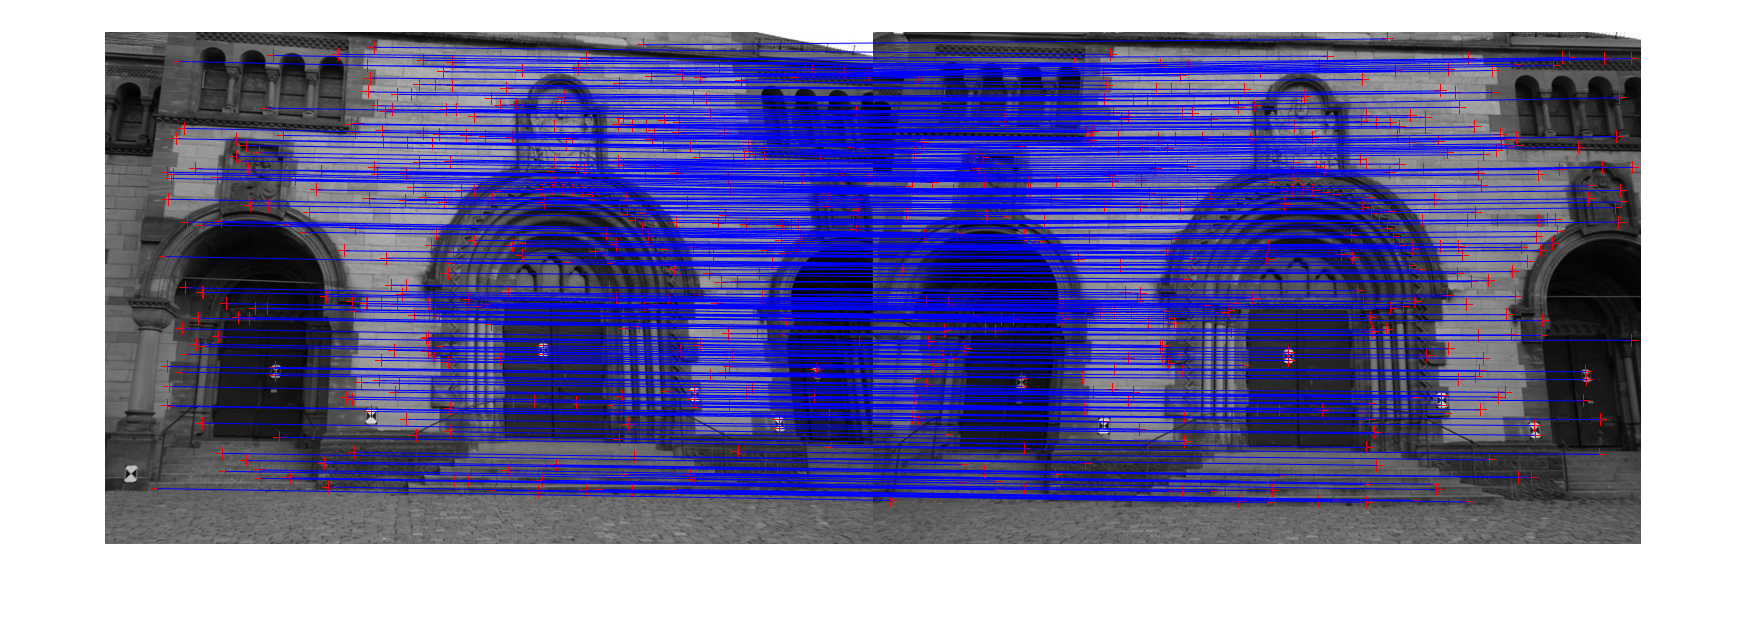
\includegraphics[width=1\linewidth, trim = {1cm 1cm 1cm 1cm}, clip]{C:/Users/Anton/Desktop/ETH_books/CV/CV-Lab-Model-Fitting/CV-Lab-Model-Fitting/img/ransac}
			\end{minipage}
		\end{center}
	\caption{Using RANSAC (threshold = 3) result is much better than with least squares and almost the same as ground truth}
	\end{figure}
\begin{center}
\begin{tabular}{|l|l|l|}
	\multicolumn{3}{c}{Errors}\\
	\hline
	\texttt{err\_ls} & \texttt{err\_ransac} & \texttt{err\_real}\\
	\hline
	134.4 & 42.5 & 41.1\\
	\hline
\end{tabular}
\end{center}
\newpage
%%%%%%%%%%%%%%%%%%%%%%%%%%%%%%%%%%%%%%%%%%%%%%%%%%%%%%%%%   2
	\textbf{2.} We implement 8-point algorithm using manually clicked points (more than 8 for better accuracy). We do everything as described in exercise task and paper <<In Defense of the Eight-Point Algorithm>>) and show epipolar lines and epipoles (found as null vectors from SVD decomposition). Below are presented results (fig. 2 -- 9).
	\begin{figure}[h]
		\begin{center}
			\begin{minipage}[h]{0.49\linewidth}
				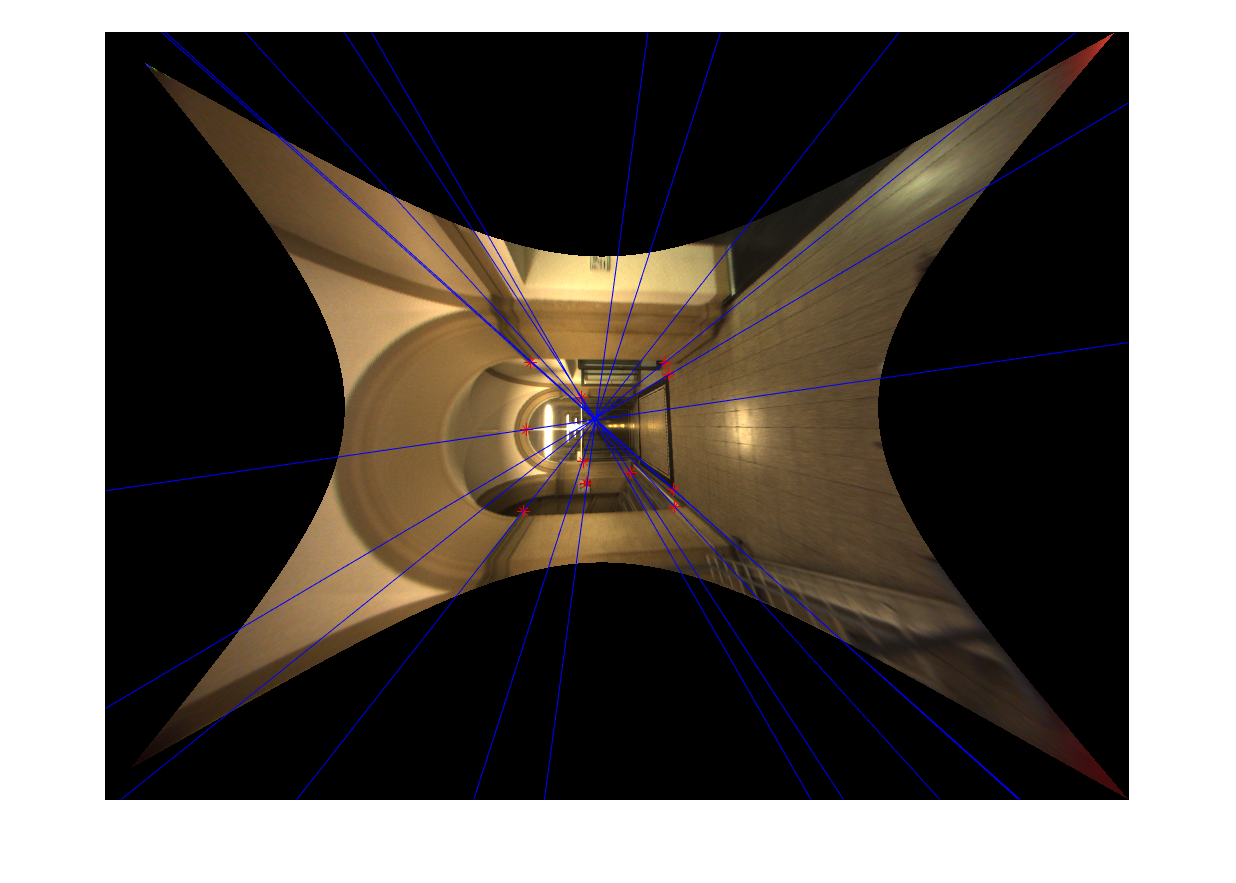
\includegraphics[width=1\linewidth, trim = {10cm 8cm 10cm 8cm}, clip]{C:/Users/Anton/Desktop/ETH_books/CV/CV-Lab-Model-Fitting/CV-Lab-Model-Fitting/src/epipolar_geometry/res/f_ladybug_1}
			\end{minipage}
			\hfill
			\begin{minipage}[h]{0.49\linewidth}
				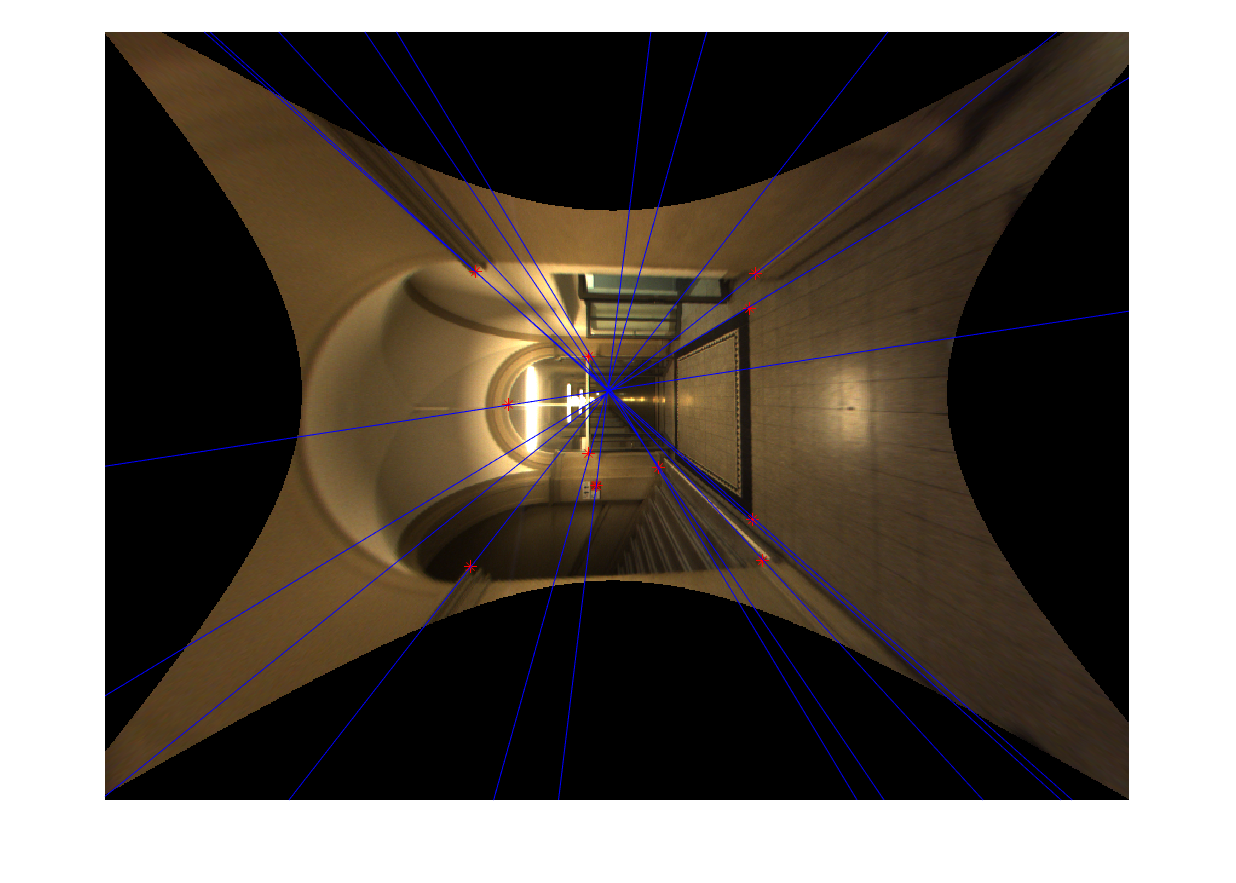
\includegraphics[width=1\linewidth, trim = {10cm 8cm 10cm 8cm}, clip]{C:/Users/Anton/Desktop/ETH_books/CV/CV-Lab-Model-Fitting/CV-Lab-Model-Fitting/src/epipolar_geometry/res/f_ladybug_2}
			\end{minipage}
		\caption{Epipolar lines and 11 used points with non-singular fundamental matrix}
		\end{center}
	\end{figure}

\begin{figure}[h]
	\begin{center}
		\begin{minipage}[h]{0.49\linewidth}
			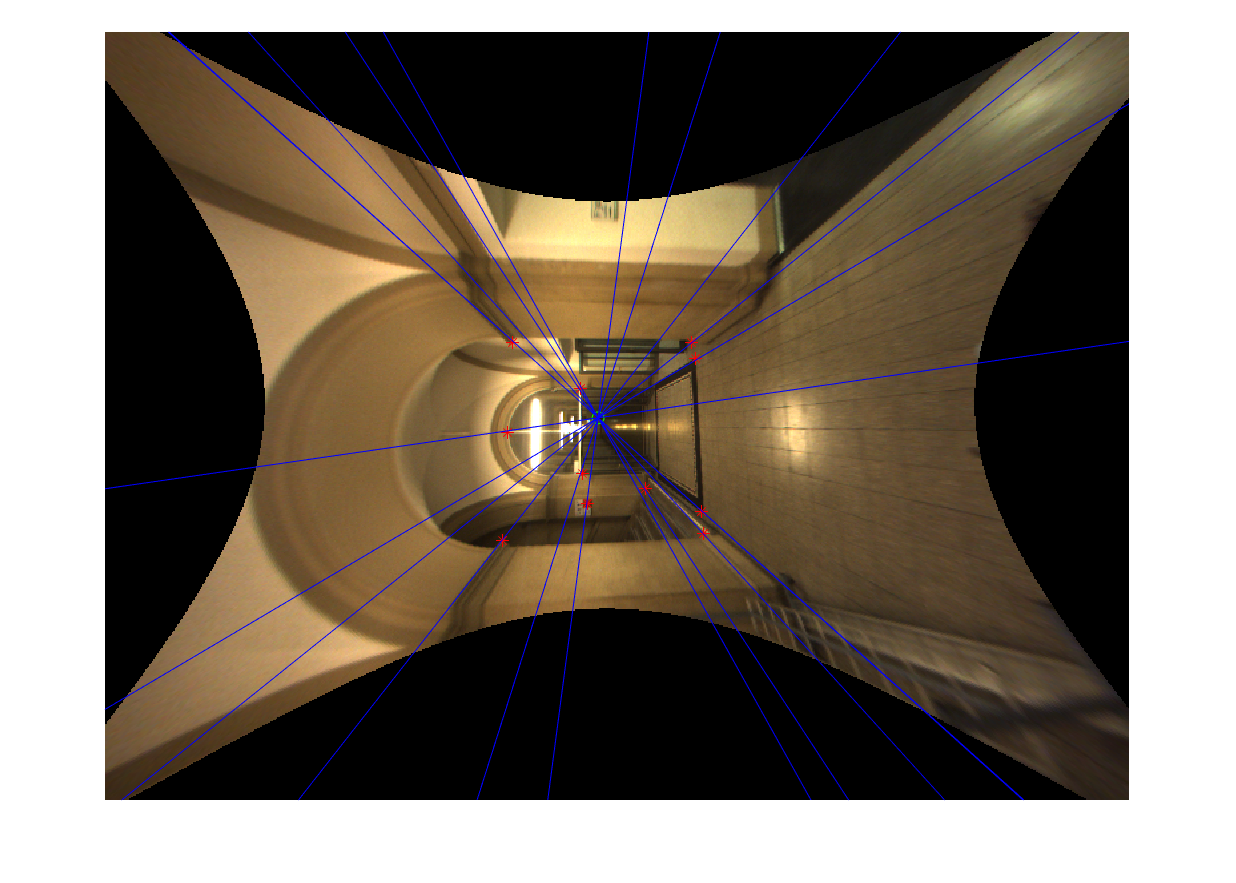
\includegraphics[width=1\linewidth, trim = {10cm 8cm 10cm 8cm}, clip]{C:/Users/Anton/Desktop/ETH_books/CV/CV-Lab-Model-Fitting/CV-Lab-Model-Fitting/src/epipolar_geometry/res/fh_ladybug_1}
			%\caption{$1,\: 0.04, \: 1\cdot10^{-6}$}%\detokenize{h_2_0.04_3e-06}
		\end{minipage}
		\hfill
		\begin{minipage}[h]{0.49\linewidth}
			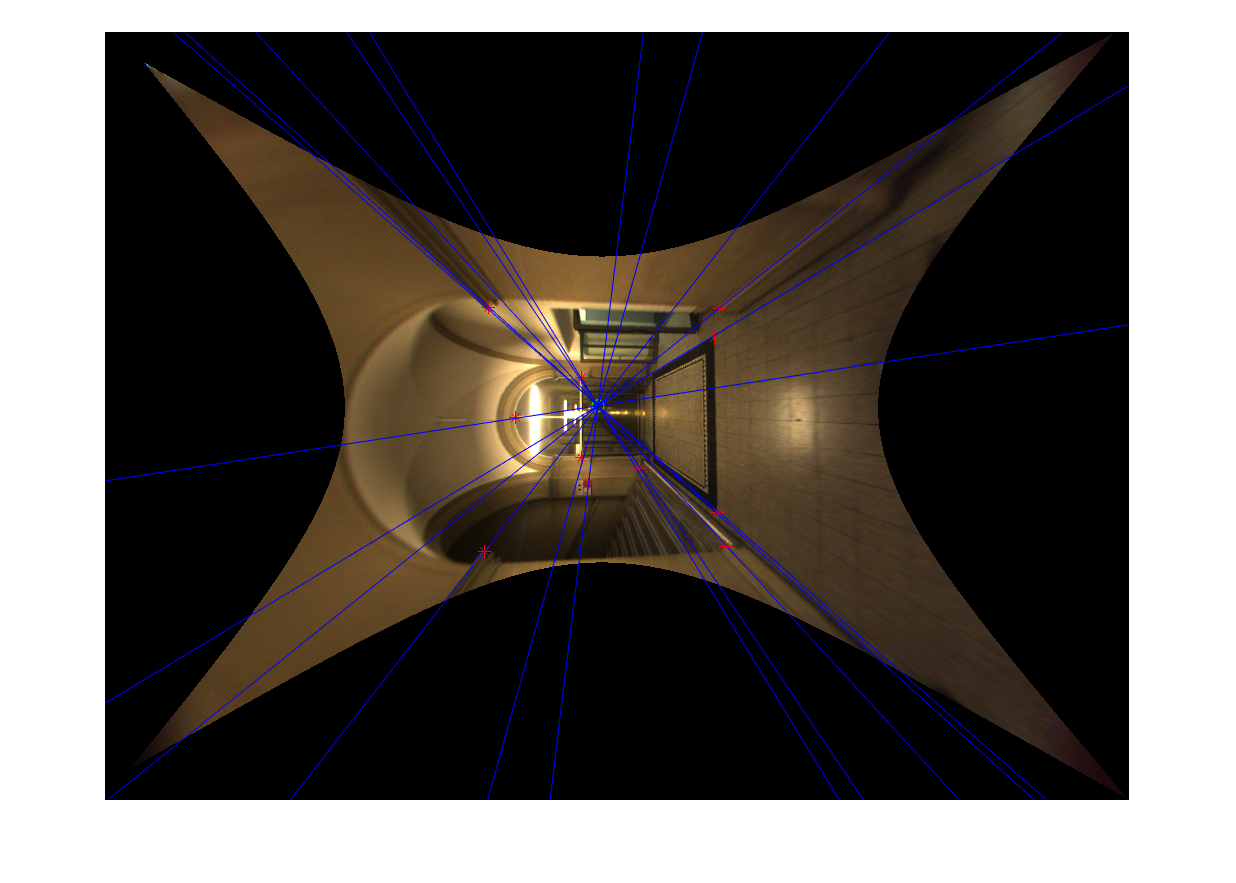
\includegraphics[width=1\linewidth, trim = {10cm 8cm 10cm 8cm}, clip]{C:/Users/Anton/Desktop/ETH_books/CV/CV-Lab-Model-Fitting/CV-Lab-Model-Fitting/src/epipolar_geometry/res/fh_ladybug_2}
		%	\caption{$1,\: 0.04, \: 3\cdot10^{-6}$}
		\end{minipage}

	\caption{Epipolar lines, epipoles (green circles) and 11 used points (red crosses) with singular fundamental matrix}
	\end{center}
\end{figure}

\begin{figure}[h!]
	\begin{center}
		\begin{minipage}[h]{0.49\linewidth}
			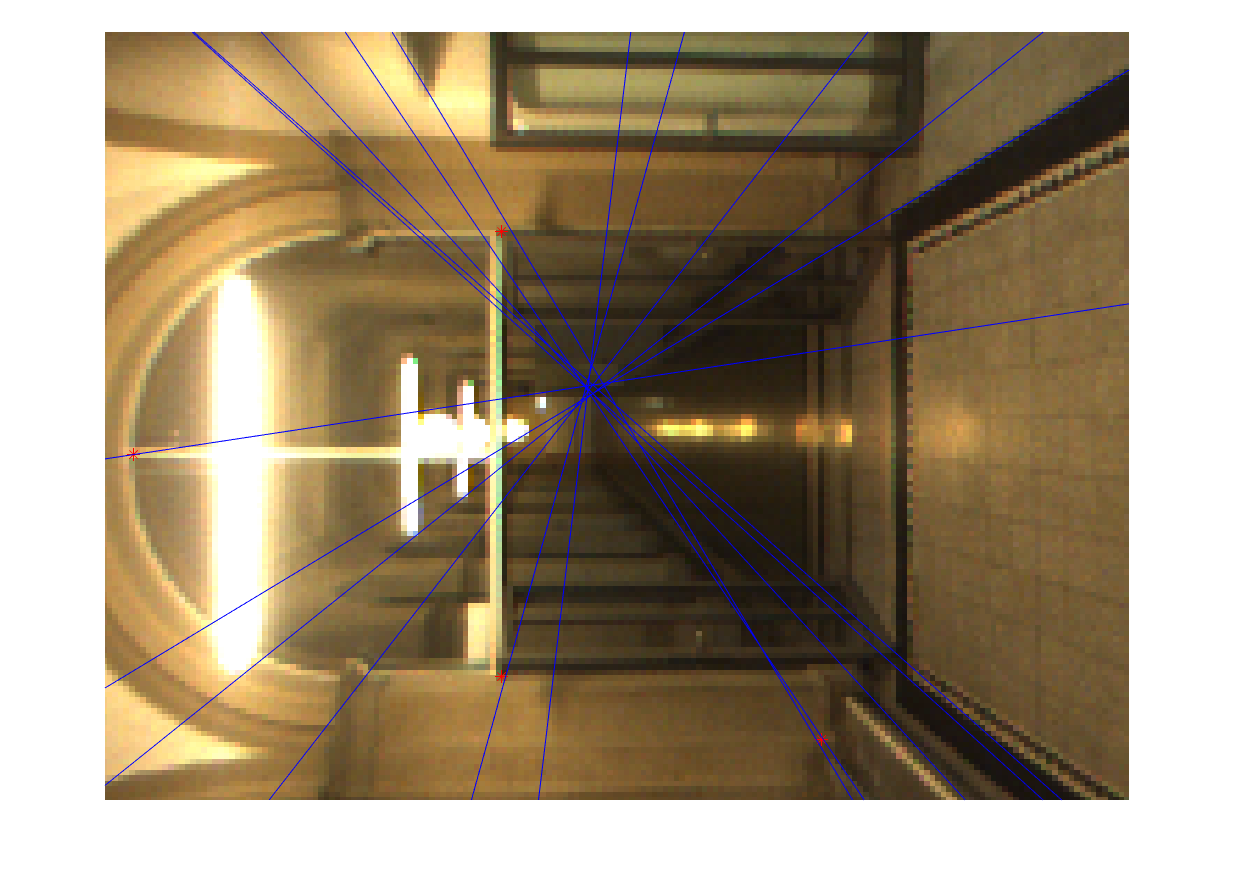
\includegraphics[width=1\linewidth, trim = {9cm 8cm 9cm 6cm}, clip]{C:/Users/Anton/Desktop/ETH_books/CV/CV-Lab-Model-Fitting/CV-Lab-Model-Fitting/src/epipolar_geometry/res/f_ladybug_3}
			%\caption{$1,\: 0.04, \: 1\cdot10^{-6}$}%\detokenize{h_2_0.04_3e-06}
		\end{minipage}
		\hfill
		\begin{minipage}[h]{0.49\linewidth}
			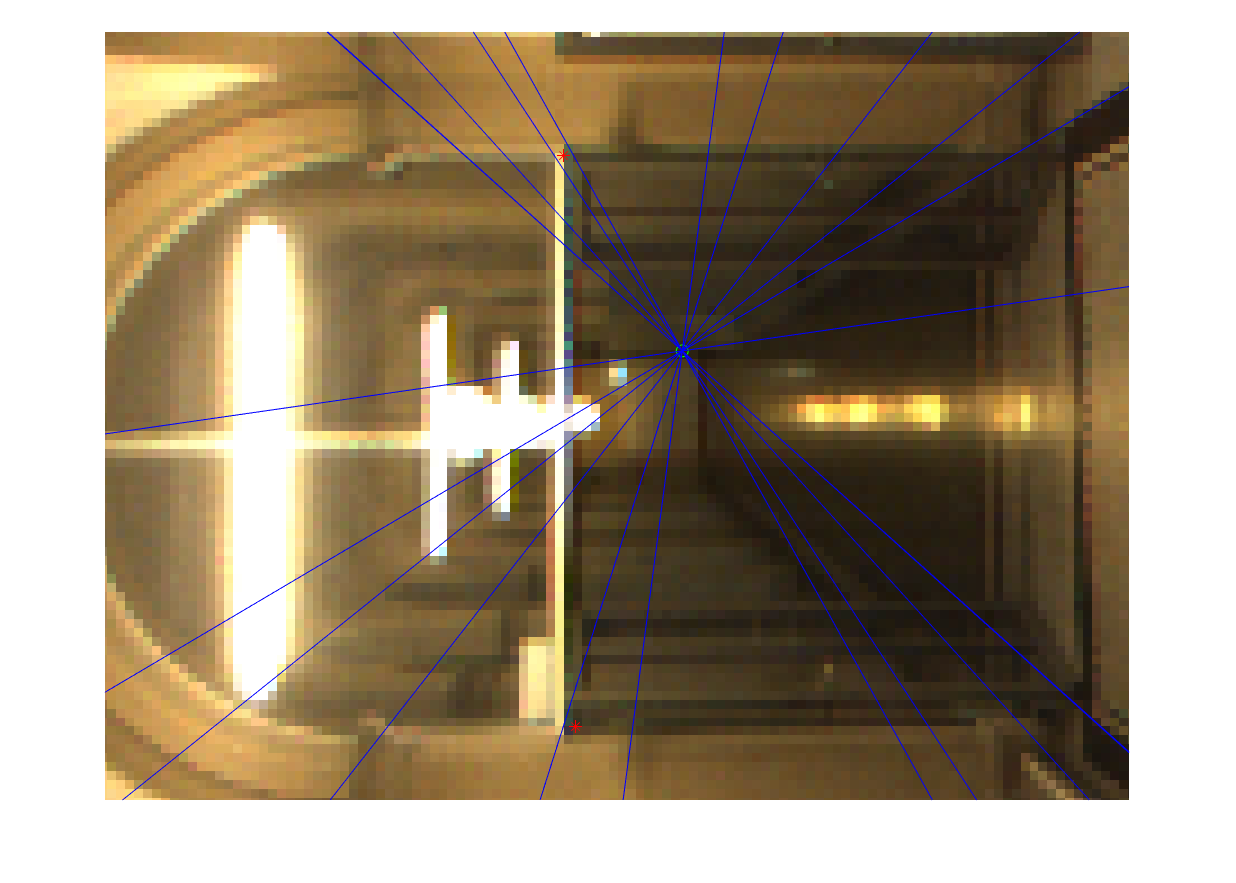
\includegraphics[width=1\linewidth, trim = {9cm 8cm 9cm 6cm}, clip]{C:/Users/Anton/Desktop/ETH_books/CV/CV-Lab-Model-Fitting/CV-Lab-Model-Fitting/src/epipolar_geometry/res/fh_ladybug_4}
			%	\caption{$1,\: 0.04, \: 3\cdot10^{-6}$}
		\end{minipage}
		
		\caption{Blowed-up intersection of epipoles, left --- with non-singularized matrix, bad; right --- with singularized matrix intersection is perfect and matches with epipole, better}
	\end{center}
\end{figure}


%%%%%%%%%%%%%%%%%%%%%%%%%%%%%%%%%%%%%%%%    pumpkin
	\begin{figure}[h]
	\begin{center}
		\begin{minipage}[h]{0.49\linewidth}
			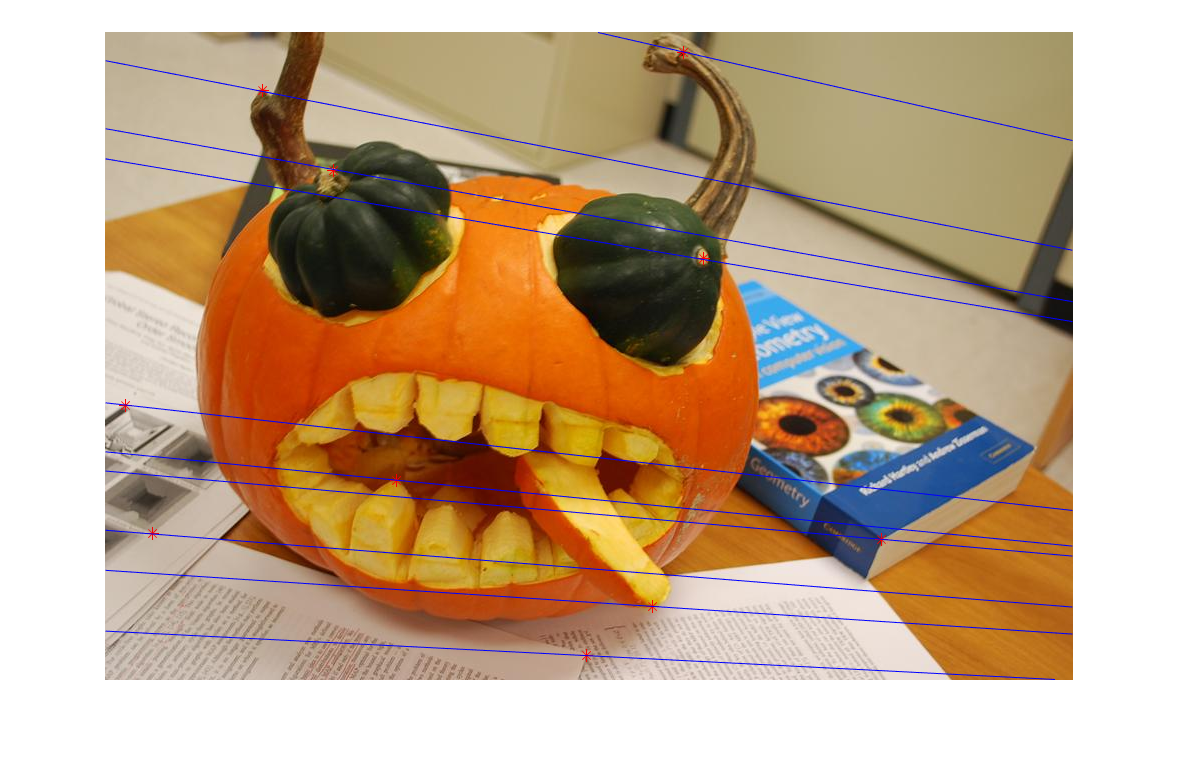
\includegraphics[width=1\linewidth, trim = {2cm 2cm 2cm 2cm}, clip]{C:/Users/Anton/Desktop/ETH_books/CV/CV-Lab-Model-Fitting/CV-Lab-Model-Fitting/src/epipolar_geometry/res/f_pumpkin_1}
		\end{minipage}
		\hfill
		\begin{minipage}[h]{0.49\linewidth}
			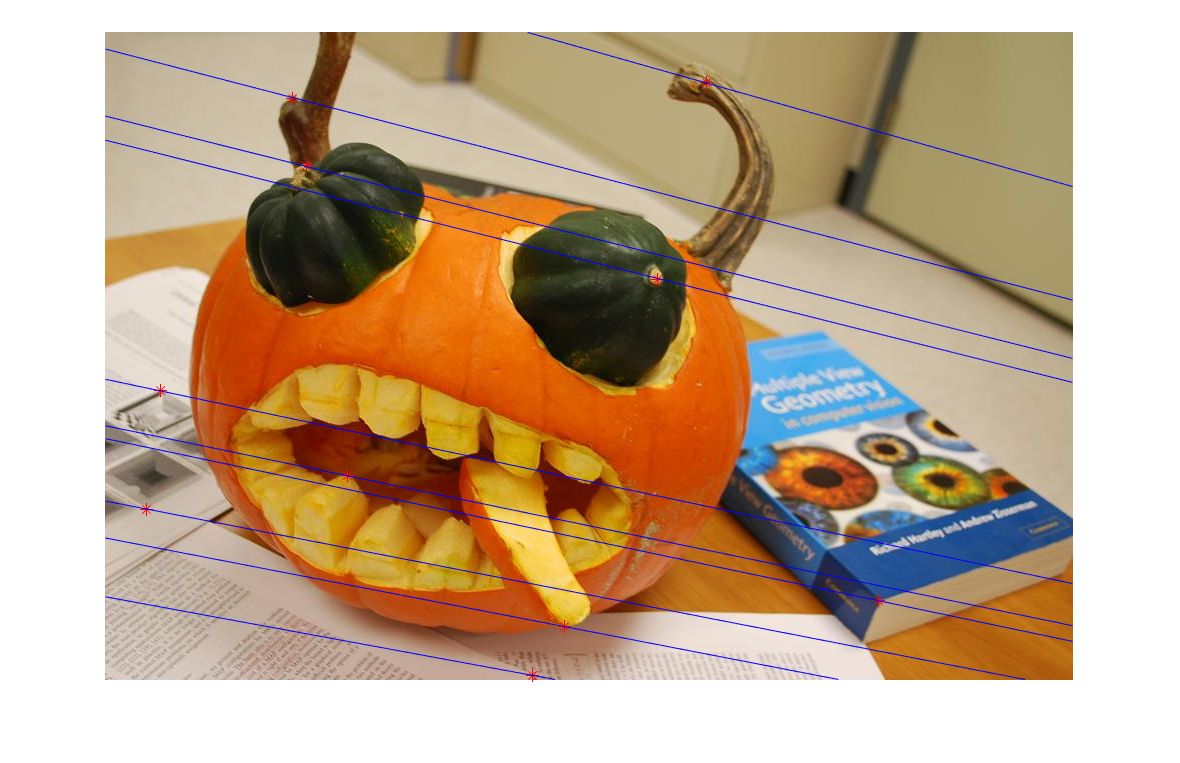
\includegraphics[width=1\linewidth, trim = {2cm 2cm 2cm 2cm}, clip]{C:/Users/Anton/Desktop/ETH_books/CV/CV-Lab-Model-Fitting/CV-Lab-Model-Fitting/src/epipolar_geometry/res/f_pumpkin_2}
		\end{minipage}
		\caption{Epipolar lines and 10 used points with non-singular fundamental matrix}
	\end{center}
\end{figure}

	\begin{figure}[h]
	\begin{center}
		\begin{minipage}[h]{0.49\linewidth}
			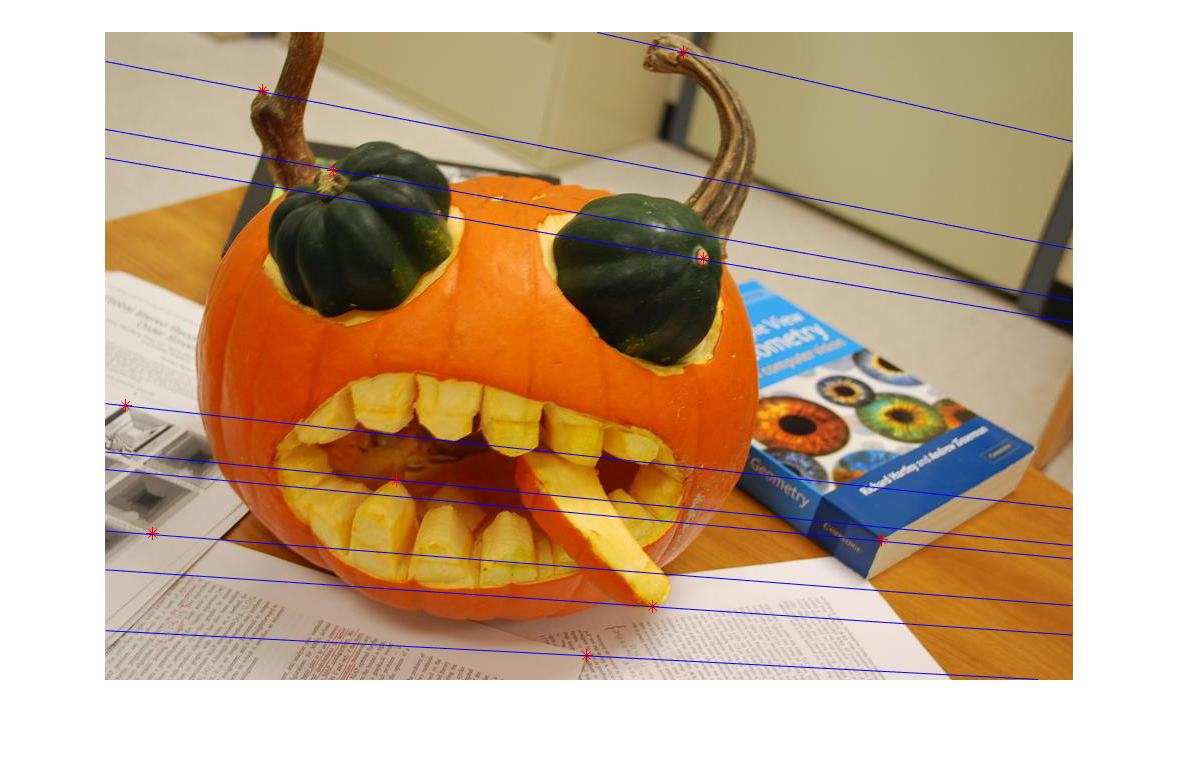
\includegraphics[width=1\linewidth, trim = {2cm 2cm 2cm 2cm}, clip]{C:/Users/Anton/Desktop/ETH_books/CV/CV-Lab-Model-Fitting/CV-Lab-Model-Fitting/src/epipolar_geometry/res/fh_pumpkin_1}
		\end{minipage}
		\hfill
		\begin{minipage}[h]{0.49\linewidth}
			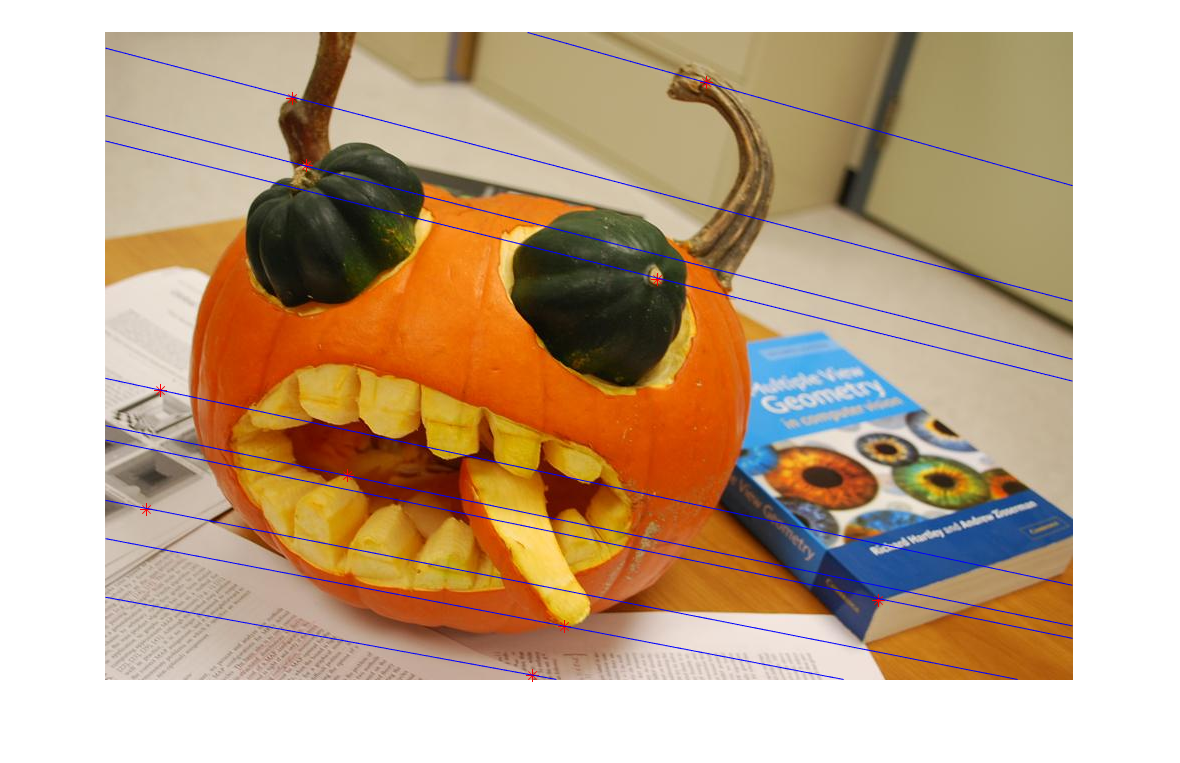
\includegraphics[width=1\linewidth, trim = {2cm 2cm 2cm 2cm}, clip]{C:/Users/Anton/Desktop/ETH_books/CV/CV-Lab-Model-Fitting/CV-Lab-Model-Fitting/src/epipolar_geometry/res/fh_pumpkin_2}
		\end{minipage}
		\caption{Epipolar lines and 10 used points with singular fundamental matrix}
	\end{center}
\end{figure}
%%%%%%%%%%%%%%%%%%%%%%%%%%%%%    rect
\begin{figure}[h!]
	\begin{center}
		\begin{minipage}[h!]{0.49\linewidth}
			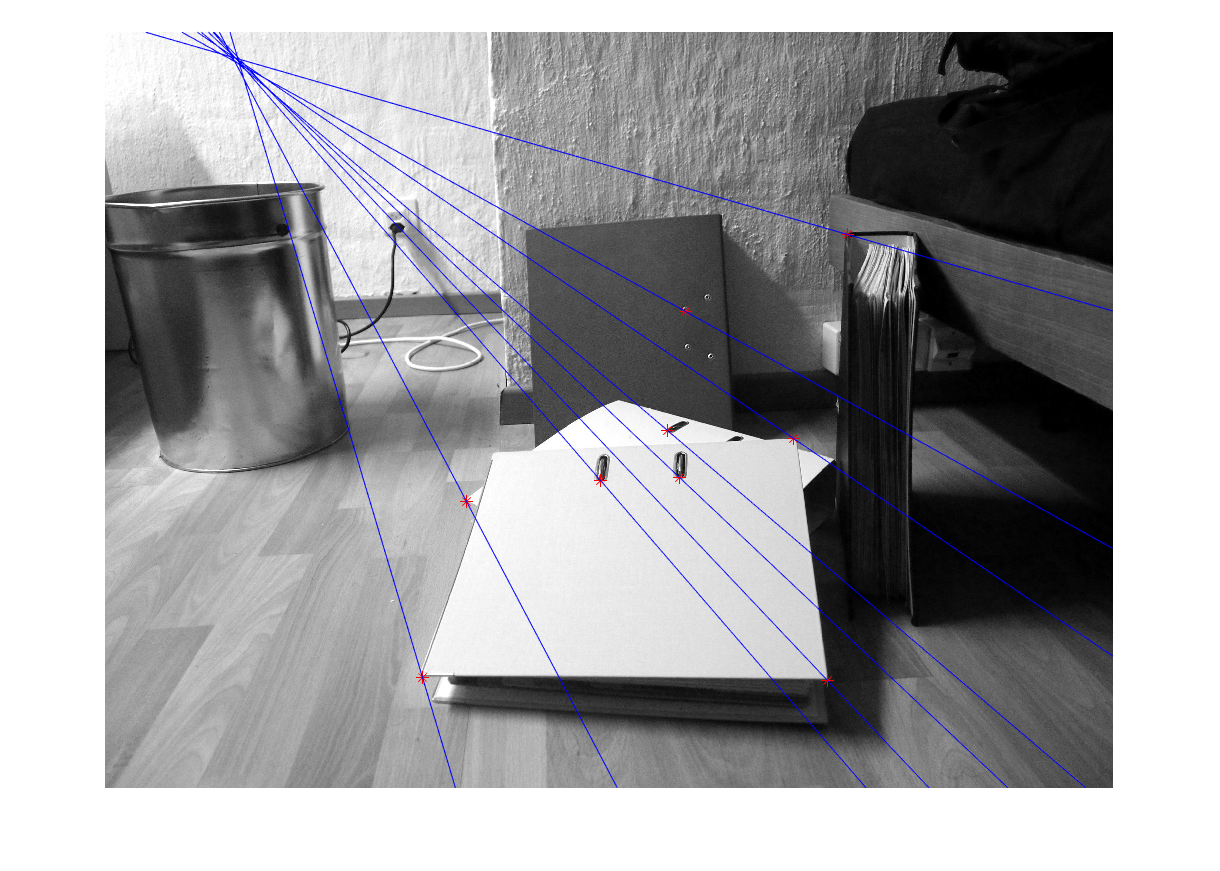
\includegraphics[width=1\linewidth, trim = {1cm 1cm 1cm 1cm}, clip]{C:/Users/Anton/Desktop/ETH_books/CV/CV-Lab-Model-Fitting/CV-Lab-Model-Fitting/src/epipolar_geometry/res/f_rect_1}
			%\caption{$1,\: 0.04, \: 1\cdot10^{-6}$}%\detokenize{h_2_0.04_3e-06}
		\end{minipage}
		\hfill
		\begin{minipage}[h!]{0.49\linewidth}
			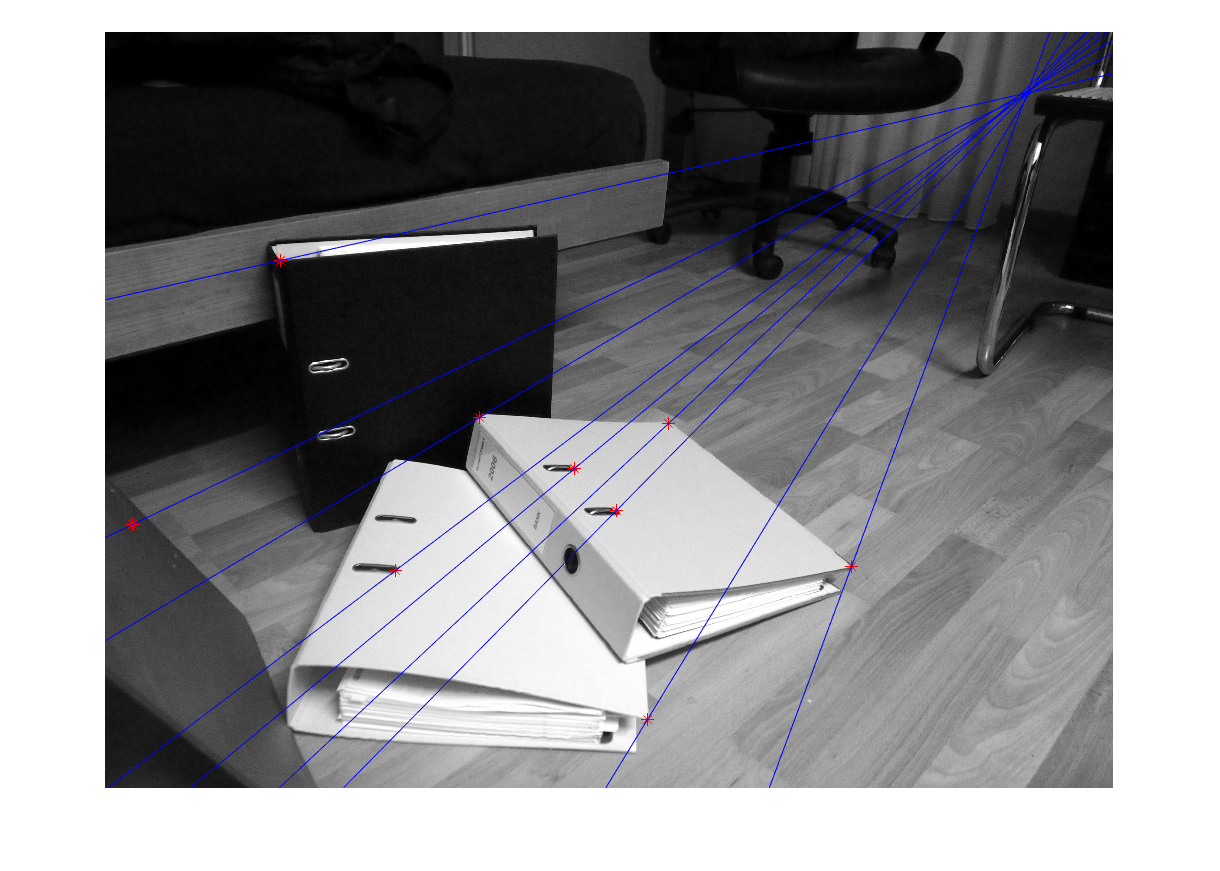
\includegraphics[width=1\linewidth, trim = {1cm 1cm 1cm 1cm}, clip]{C:/Users/Anton/Desktop/ETH_books/CV/CV-Lab-Model-Fitting/CV-Lab-Model-Fitting/src/epipolar_geometry/res/f_rect_2}
			%	\caption{$1,\: 0.04, \: 3\cdot10^{-6}$}
		\end{minipage}
		
		\caption{Epipolar lines and 9 used points with non-singular fundamental matrix}
	\end{center}
\end{figure}

\begin{figure}[h!]
	\begin{center}
		\begin{minipage}[h!]{0.49\linewidth}
			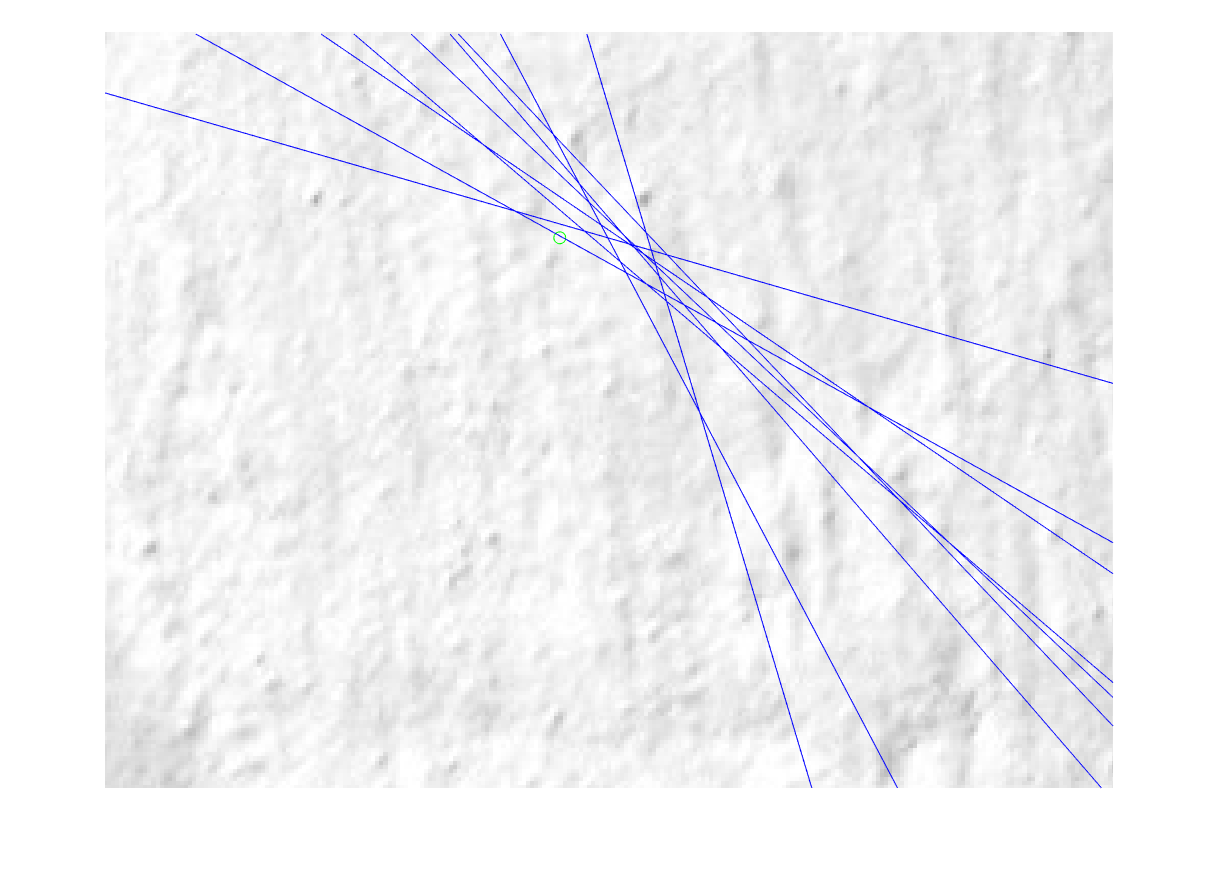
\includegraphics[width=1\linewidth, trim = {1cm 1cm 1cm 1cm}, clip]{C:/Users/Anton/Desktop/ETH_books/CV/CV-Lab-Model-Fitting/CV-Lab-Model-Fitting/src/epipolar_geometry/res/f_rect_3}
			%\caption{$1,\: 0.04, \: 1\cdot10^{-6}$}%\detokenize{h_2_0.04_3e-06}
		\end{minipage}
		\hfill
		\begin{minipage}[h!]{0.49\linewidth}
			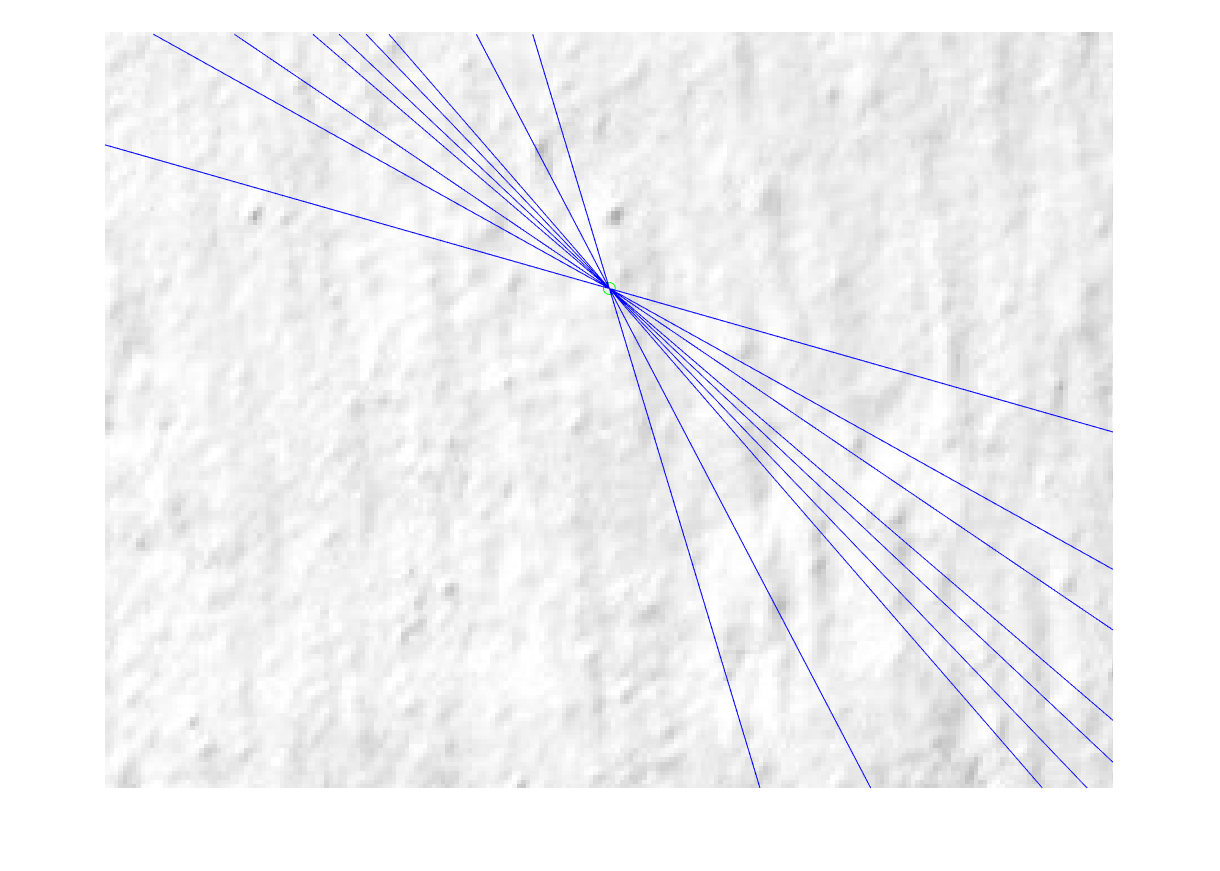
\includegraphics[width=1\linewidth, trim = {1cm 1cm 1cm 1cm}, clip]{C:/Users/Anton/Desktop/ETH_books/CV/CV-Lab-Model-Fitting/CV-Lab-Model-Fitting/src/epipolar_geometry/res/fh_rect_6}
			%	\caption{$1,\: 0.04, \: 3\cdot10^{-6}$}
		\end{minipage}
		
		\caption{Blowed-up intersection of epipoles, left --- with non-singularized matrix, bad; right --- with singularized matrix intersection is perfect and matches with epipole, better}
	\end{center}
\end{figure}

\begin{figure}[h!]
	\begin{center}
		\begin{minipage}[h!]{0.49\linewidth}
			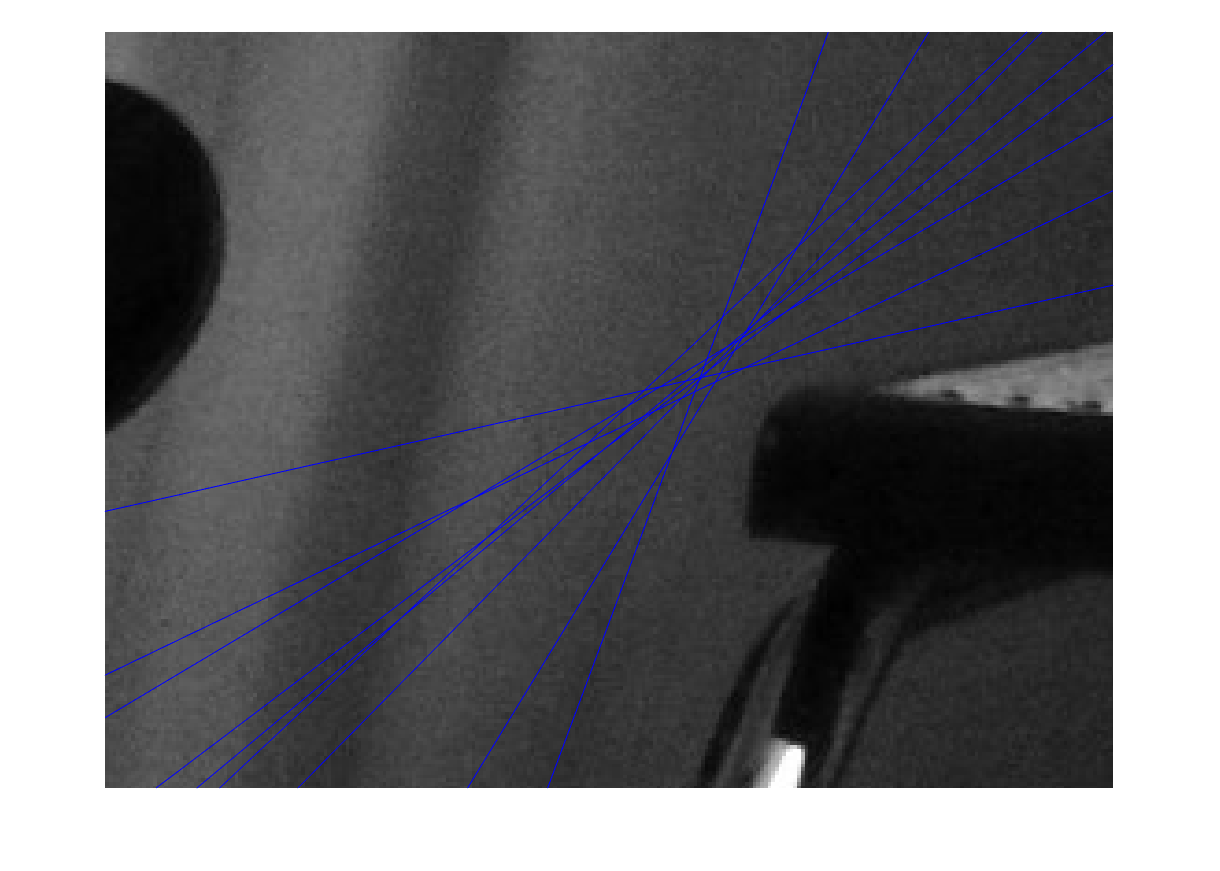
\includegraphics[width=1\linewidth, trim = {1cm 1cm 1cm 1cm}, clip]{C:/Users/Anton/Desktop/ETH_books/CV/CV-Lab-Model-Fitting/CV-Lab-Model-Fitting/src/epipolar_geometry/res/f_rect_4}
			%\caption{$1,\: 0.04, \: 1\cdot10^{-6}$}%\detokenize{h_2_0.04_3e-06}
		\end{minipage}
		\hfill
		\begin{minipage}[h!]{0.49\linewidth}
			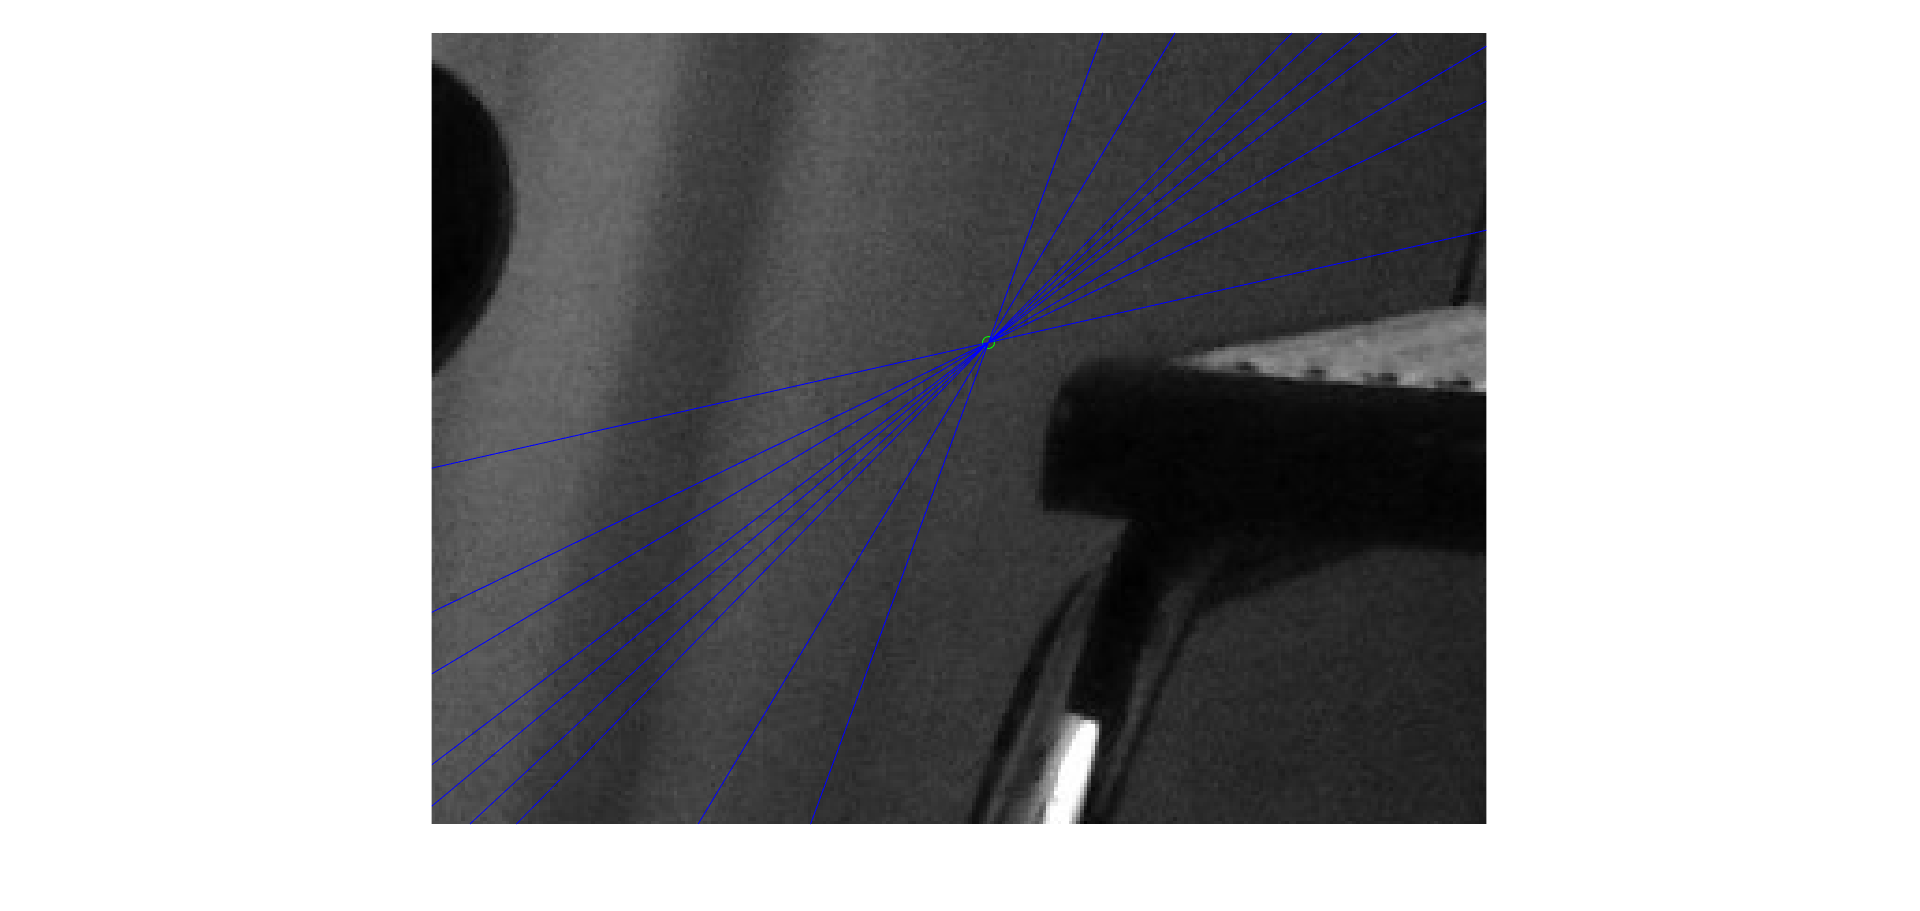
\includegraphics[width=1\linewidth, trim = {12cm 3cm 12cm 3cm}, clip]{C:/Users/Anton/Desktop/ETH_books/CV/CV-Lab-Model-Fitting/CV-Lab-Model-Fitting/src/epipolar_geometry/res/fh_rect_5}
			%	\caption{$1,\: 0.04, \: 3\cdot10^{-6}$}
		\end{minipage}
		
		\caption{Blowed-up intersection of epipoles, left --- with non-singularized matrix, bad; right --- with singularized matrix intersection is perfect and matches with epipole, better}
	\end{center}
\end{figure}
%%%%%%%%%%%%%%%%%%%%%%%%%%%%%%%%%%%%%%%%%%%%%%%%%%%%%%%%%   3
	\newpage
	\newpage
	\newpage
	\textbf{3.} We download and extract vlfeat to the working directory, initialize it using \\
	\texttt{run(strcat(pwd, '/vlfeat-0.9.21/toolbox/vl\_setup'));}\\
	and run \texttt{main\_ransac8pF.m} without the second <<ransac>> part. Result at the fig. 10
	\begin{figure}[h!]
		\begin{center}
			\begin{minipage}[h]{0.9\linewidth}
				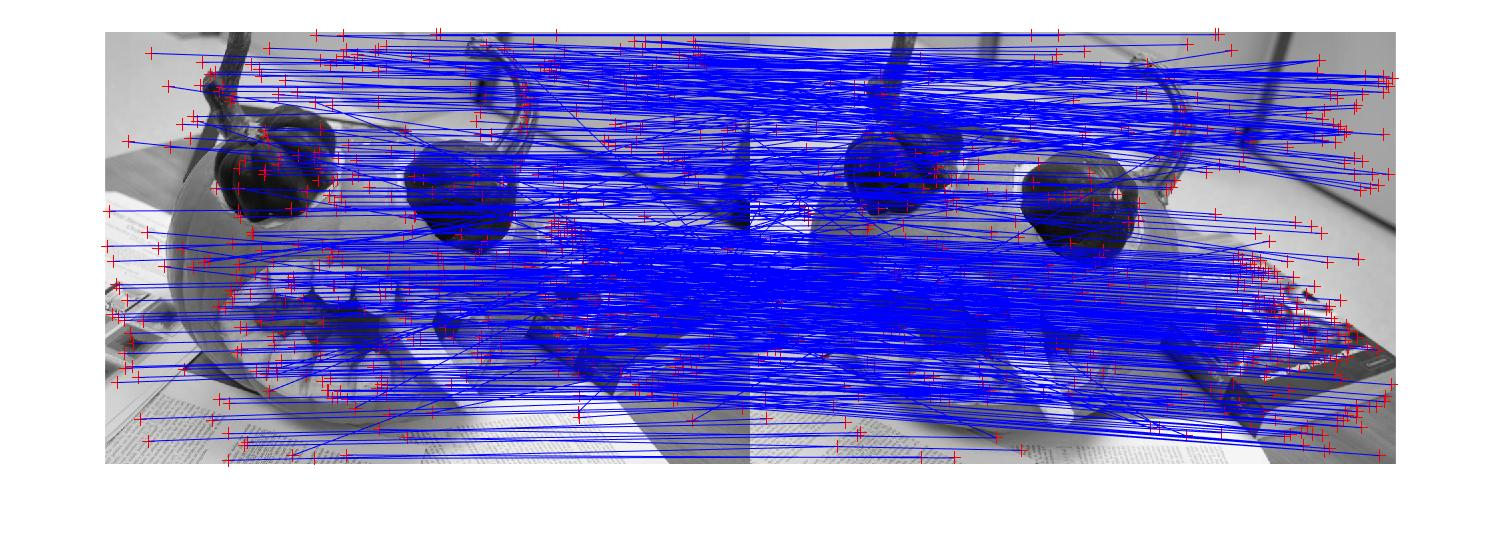
\includegraphics[width=1\linewidth, trim = {1cm 1cm 1cm 1cm}, clip]{C:/Users/Anton/Desktop/ETH_books/CV/CV-Lab-Model-Fitting/CV-Lab-Model-Fitting/src/epipolar_geometry/res/vlfeat}
				\caption{SIFT matching using vlfeat, many inaccuracies present (at least too diagonal lines)}
			\end{minipage}
			\end{center}
	\end{figure}
%%%%%%%%%%%%%%%%%%%%%%%%%%%%%%%%%%%%%%%%%%%%%%%%%%%%%%%%%   4
	\newpage
	\textbf{4.} Choose random 8 points from output of vlfeat, find singular fundamental matrix $\hat{F}$ and using it implement RANSAC algorithm on all the points of interest with different threshold. Distance is measured as sum of orthonormal distances from every point in pair to the epipolar line generated by other point from the pair:%(from article <<In Defense of the Eight-Point Algorithm>>, p.585, right-up)
	$$\mathcal{S}(x,x') = d(x', Fx) + d(x, F^\top x'),$$ where
	$$ d(x_2, Fx_1) = \dfrac{x_2^\top Fx_1}{\sqrt{a^2+b^2}} \:\text{if}\:Fx_1 = (a, b, c)^\top \iff \:\text{epipolar line}\:\{ax+by+c=0\}$$
	Results at the figures 11 ~-- 27. Seeing the pictures and trying to conclude, we can propose, that the most balanced result is achieved when threshold is about 10\% of dimensions of the image (if it's more or less quadratic).
	\begin{figure}[h!]
		\begin{center}
			\begin{minipage}[h]{0.9\linewidth}
				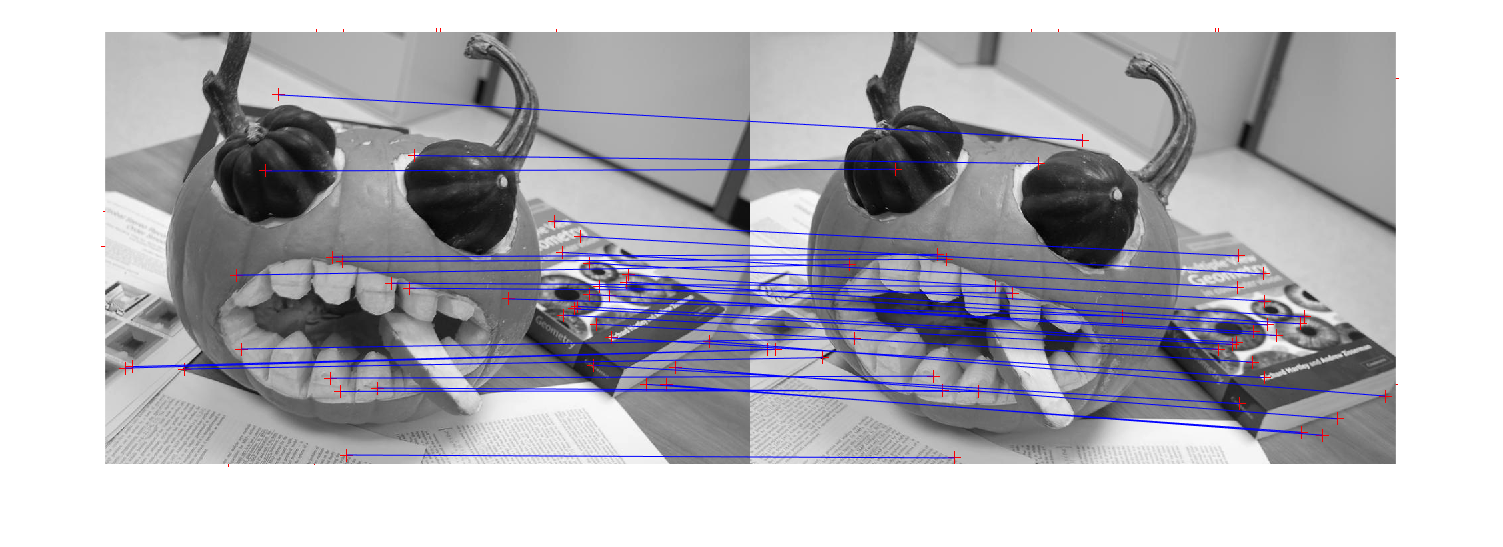
\includegraphics[width=1\linewidth, trim = {3cm 1cm 3cm 1cm}, clip]{C:/Users/Anton/Desktop/ETH_books/CV/CV-Lab-Model-Fitting/CV-Lab-Model-Fitting/src/epipolar_geometry/res/z-02-1000}
				\caption{RANSAC, 0.2 threshold, 1000 iterations. Maybe, too small number of inliers}
			\end{minipage}
		\end{center}
	\end{figure} 
	\begin{figure}[h!]
		\begin{center}
			\begin{minipage}[h]{0.9\linewidth}
				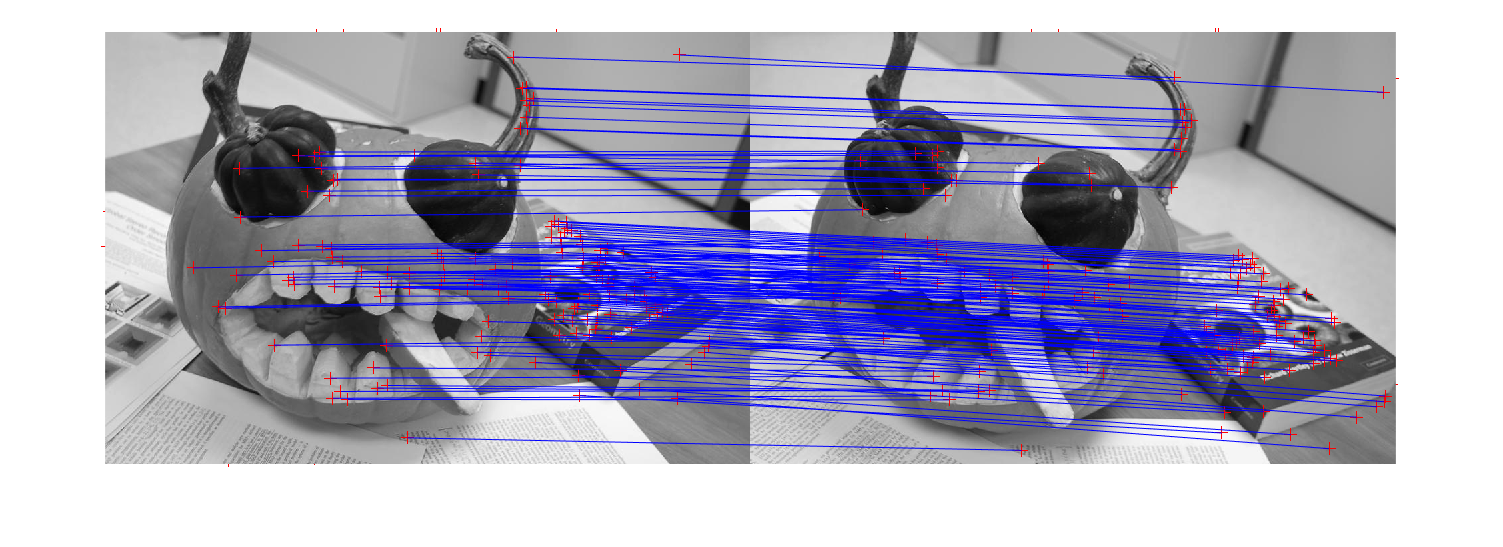
\includegraphics[width=1\linewidth, trim = {3cm 1cm 3cm 1cm}, clip]{C:/Users/Anton/Desktop/ETH_books/CV/CV-Lab-Model-Fitting/CV-Lab-Model-Fitting/src/epipolar_geometry/res/z-1-1000}
				\caption{RANSAC, 1 threshold, 1000 iterations. Better, but still a few of inliers}
			\end{minipage}
		\end{center}
	\end{figure}
		\begin{figure}[h!]
		\begin{center}
			\begin{minipage}[h]{0.9\linewidth}
				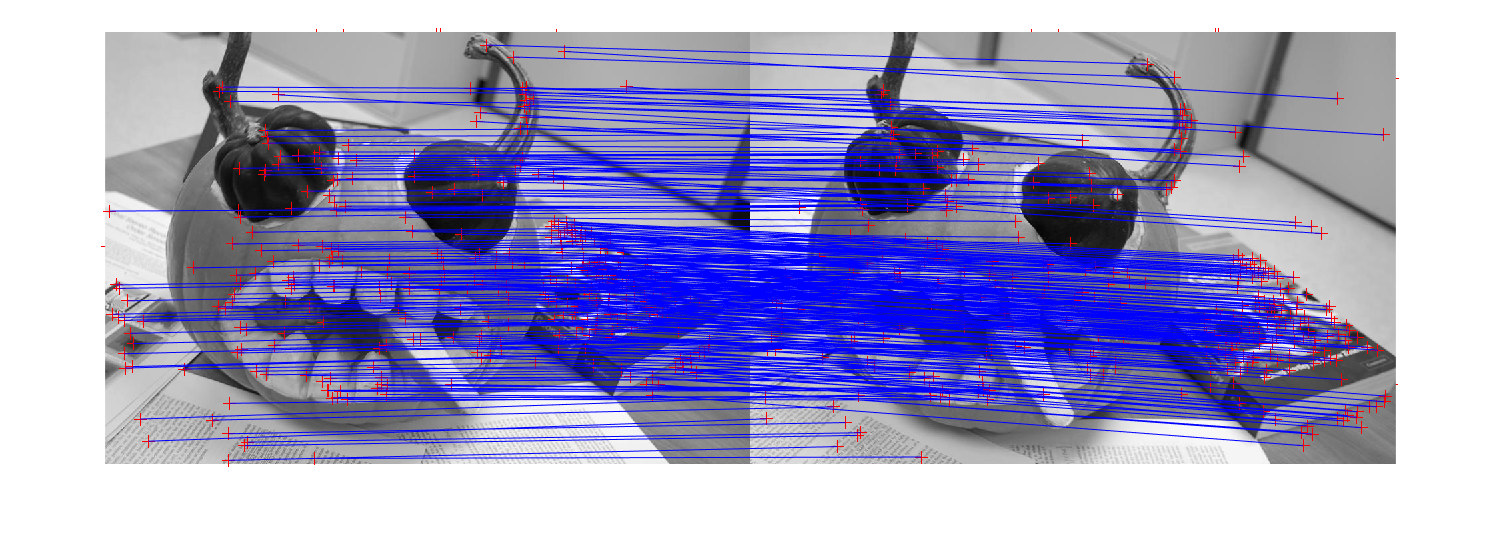
\includegraphics[width=1\linewidth, trim = {3cm 1cm 3cm 1cm}, clip]{C:/Users/Anton/Desktop/ETH_books/CV/CV-Lab-Model-Fitting/CV-Lab-Model-Fitting/src/epipolar_geometry/res/z-5-1000}
				\caption{RANSAC, 5 threshold, 1000 iterations. Looks good}
			\end{minipage}
		\end{center}
	\end{figure}
	
	\begin{figure}[h!]
		\begin{center}
			\begin{minipage}[h]{0.9\linewidth}
				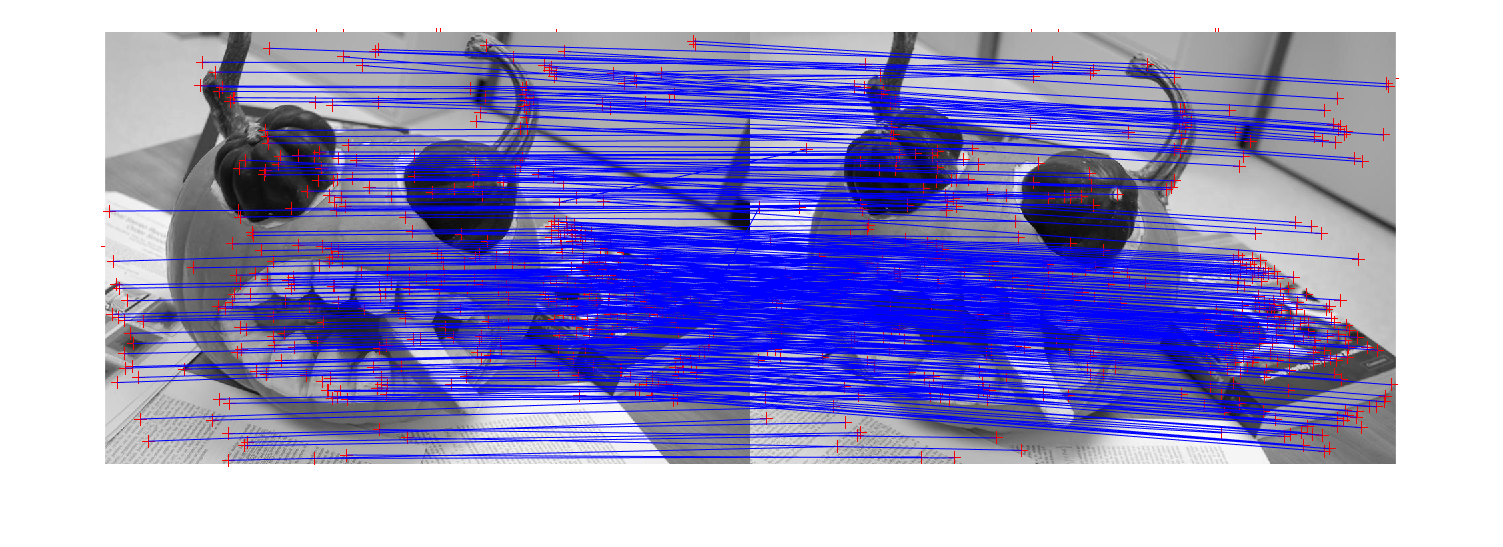
\includegraphics[width=1\linewidth, trim = {3cm 1cm 3cm 1cm}, clip]{C:/Users/Anton/Desktop/ETH_books/CV/CV-Lab-Model-Fitting/CV-Lab-Model-Fitting/src/epipolar_geometry/res/z-20-1000}
				\caption{RANSAC, 20 threshold, 1000 iterations. Now, probably, too many errors, but ok}
			\end{minipage}
		\end{center}
	\end{figure}

\begin{figure}[h!]
	\begin{center}
		\begin{minipage}[h]{0.9\linewidth}
			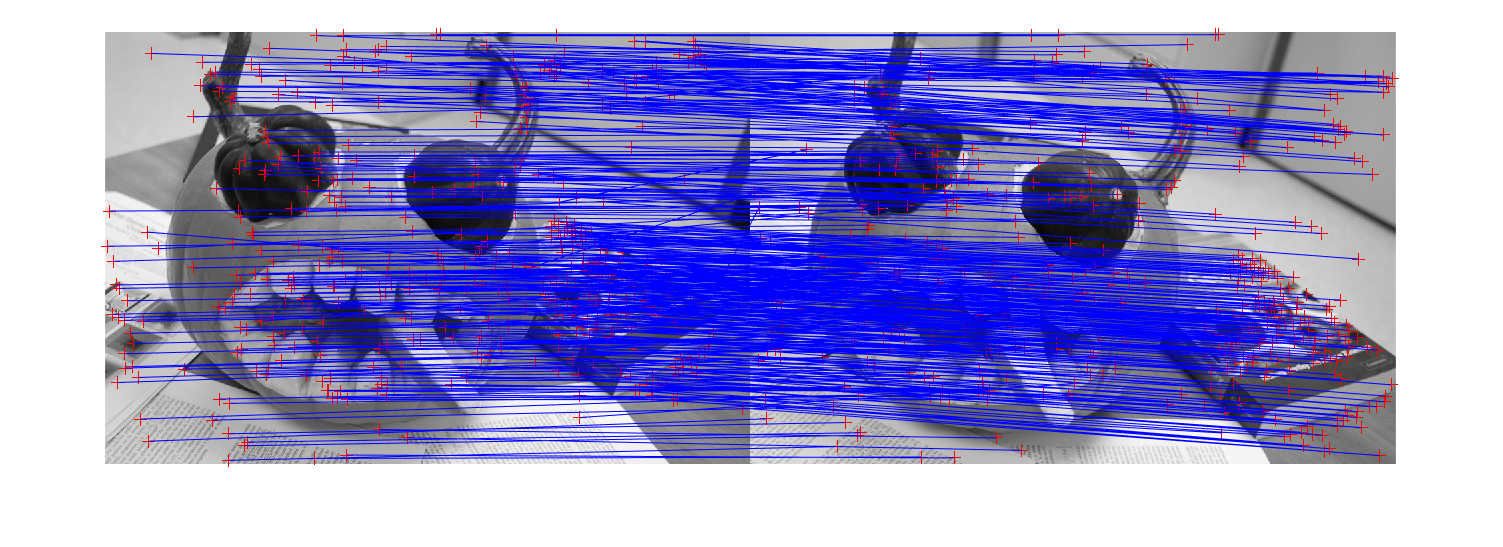
\includegraphics[width=1\linewidth, trim = {3cm 1cm 3cm 1cm}, clip]{C:/Users/Anton/Desktop/ETH_books/CV/CV-Lab-Model-Fitting/CV-Lab-Model-Fitting/src/epipolar_geometry/res/z-100-1000}
			\caption{RANSAC, 100 threshold, 1000 iterations. Almost all points in inliers, not so good among points in clusters}
		\end{minipage}
	\end{center}
\end{figure}	

\begin{center}
	\begin{tabular}{|l|l|l|l|l|l|}
		\multicolumn{4}{c}{Statistics of RANSAC 8 points algorithm (pumpkin),}\\
		 \multicolumn{4}{c}{1000 iterations, 630 points }\\
		 
		\hline
		\texttt{threshold} &0.2&1 & 5 & 20 & 100 \\
		\hline
	inliers&43&172&353 & 446 &532 \\
	\hline 	
	mean Sampson dist &0.09&0.48&1.67&4.26&15.9 \\
		\hline
	inliers/mean Sampson dist &486&357& 212& 105 & 33\\ \hline
	\end{tabular}
\end{center}

%%%%%%%%%%%%%%%%%%%%%%%%%%%%%%   BOOK
	\begin{figure}[h!]
	\begin{center}
		\begin{minipage}[h]{0.9\linewidth}
			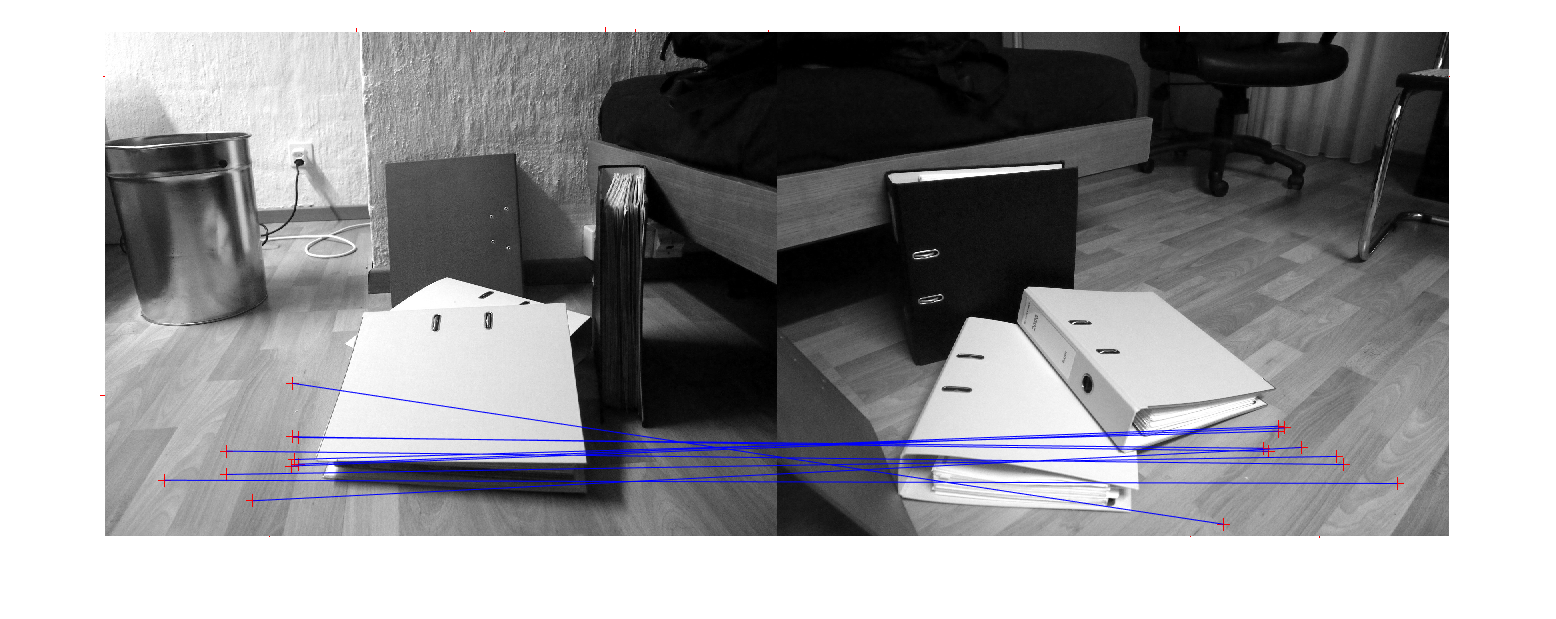
\includegraphics[width=1\linewidth, trim = {3cm 1cm 3cm 1cm}, clip]{C:/Users/Anton/Desktop/ETH_books/CV/CV-Lab-Model-Fitting/CV-Lab-Model-Fitting/src/epipolar_geometry/res/y-02-1000}
			\caption{RANSAC, 0.2 threshold, 1000 iterations.}
		\end{minipage}
	\end{center}
\end{figure} 
\begin{figure}[h!]
	\begin{center}
		\begin{minipage}[h]{0.9\linewidth}
			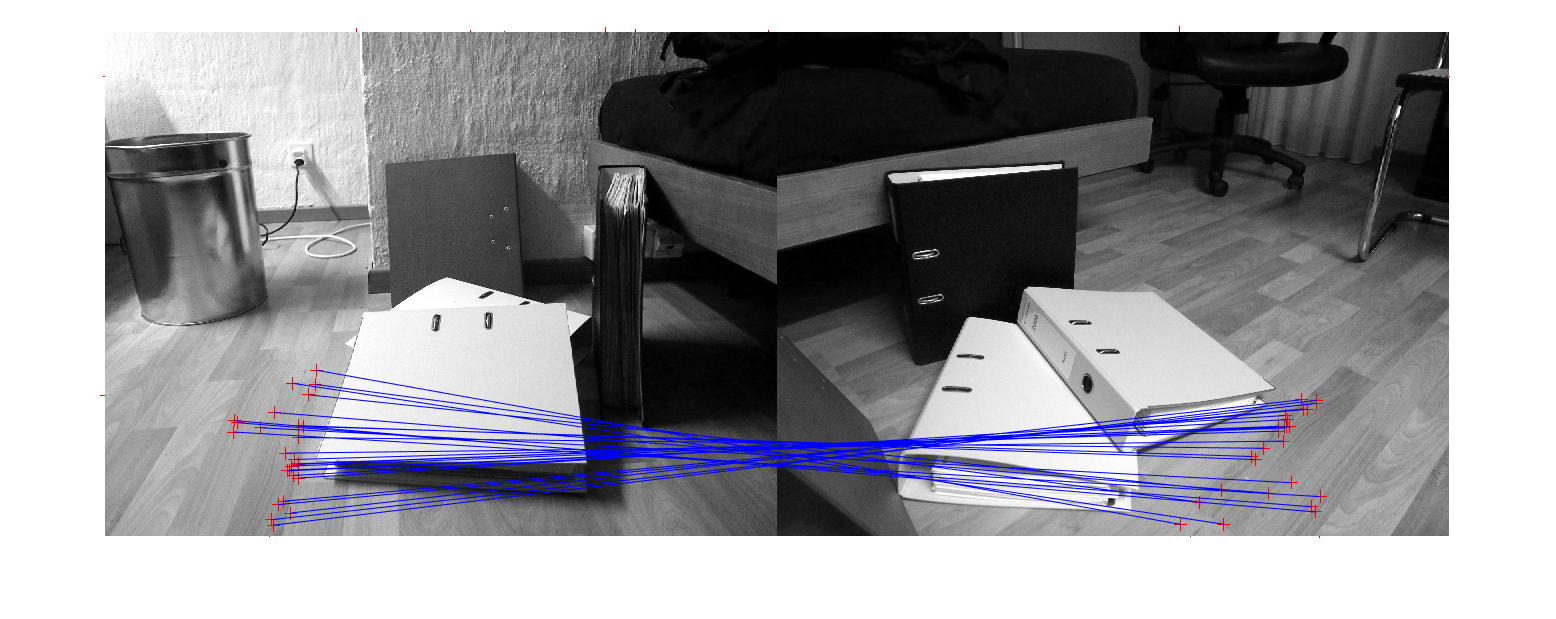
\includegraphics[width=1\linewidth, trim = {3cm 1cm 3cm 1cm}, clip]{C:/Users/Anton/Desktop/ETH_books/CV/CV-Lab-Model-Fitting/CV-Lab-Model-Fitting/src/epipolar_geometry/res/y-1-1000}
			\caption{RANSAC, 1 threshold, 1000 iterations.}
		\end{minipage}
	\end{center}
\end{figure}
\begin{figure}[h!]
	\begin{center}
		\begin{minipage}[h]{0.9\linewidth}
			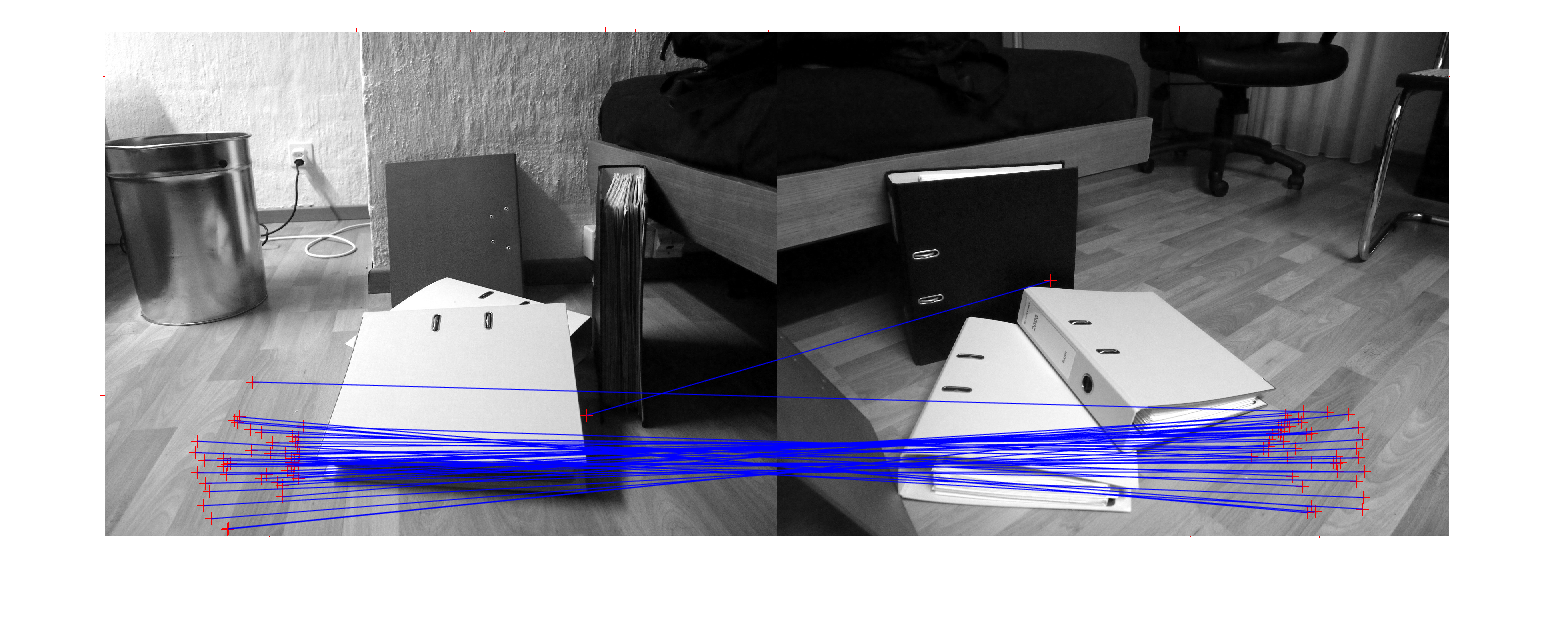
\includegraphics[width=1\linewidth, trim = {3cm 1cm 3cm 1cm}, clip]{C:/Users/Anton/Desktop/ETH_books/CV/CV-Lab-Model-Fitting/CV-Lab-Model-Fitting/src/epipolar_geometry/res/y-5-1000}
			\caption{RANSAC, 5 threshold, 1000 iterations.}
		\end{minipage}
	\end{center}
\end{figure}

\begin{figure}[h!]
	\begin{center}
		\begin{minipage}[h]{0.9\linewidth}
			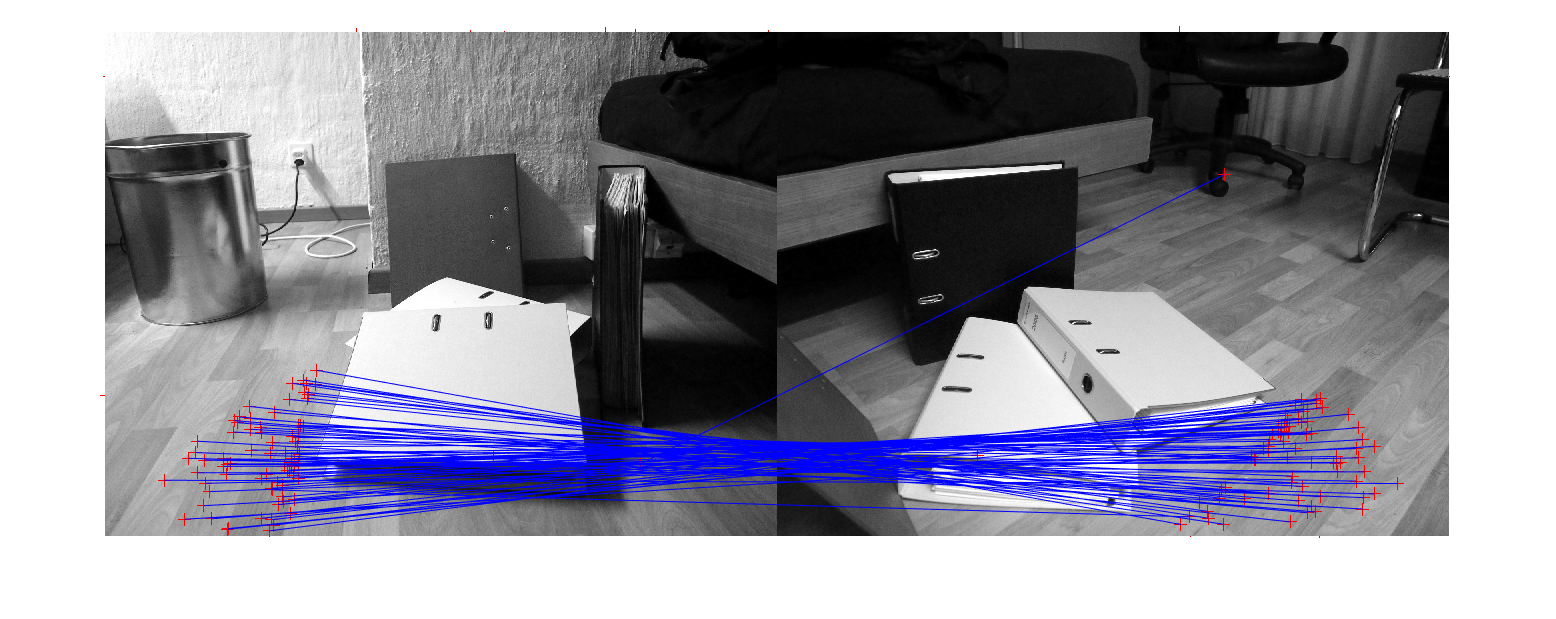
\includegraphics[width=1\linewidth, trim = {3cm 1cm 3cm 1cm}, clip]{C:/Users/Anton/Desktop/ETH_books/CV/CV-Lab-Model-Fitting/CV-Lab-Model-Fitting/src/epipolar_geometry/res/y-20-1000}
			\caption{RANSAC, 20 threshold, 1000 iterations.}
		\end{minipage}
	\end{center}
\end{figure}

\begin{figure}[h!]
	\begin{center}
		\begin{minipage}[h]{0.9\linewidth}
			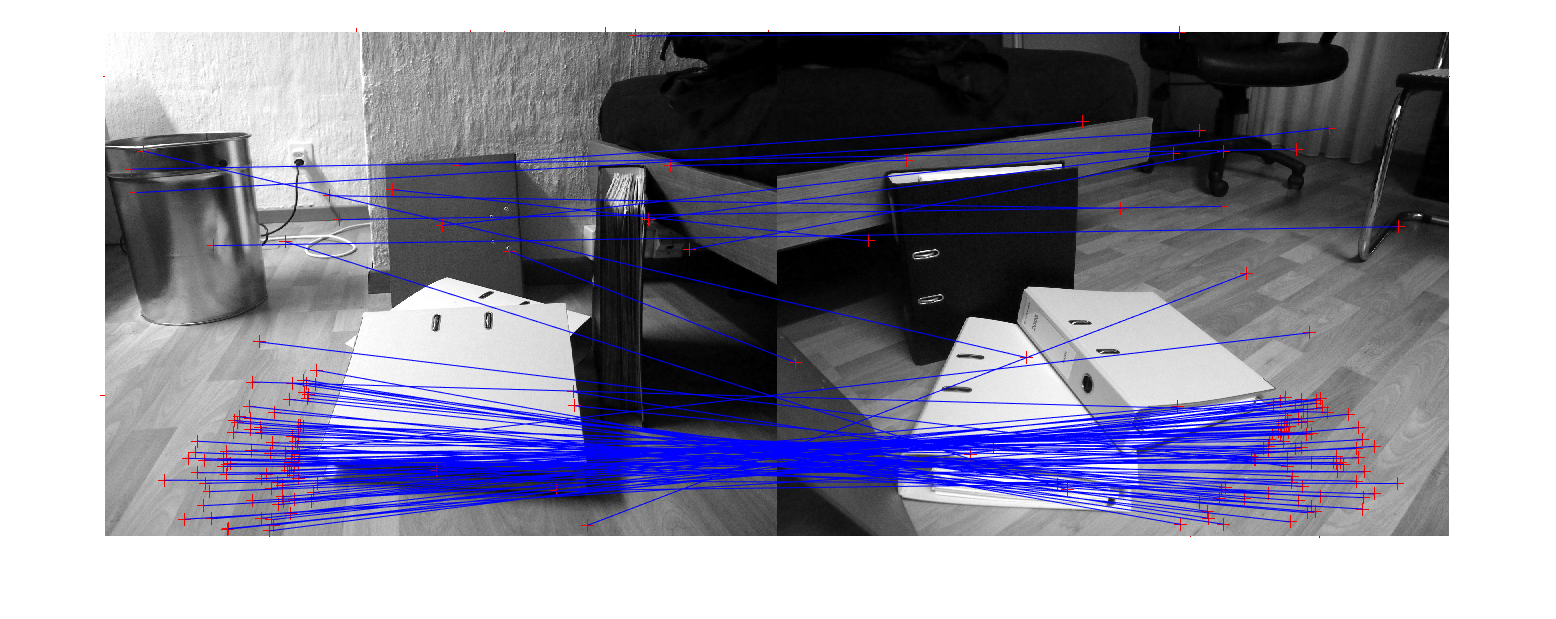
\includegraphics[width=1\linewidth, trim = {3cm 1cm 3cm 1cm}, clip]{C:/Users/Anton/Desktop/ETH_books/CV/CV-Lab-Model-Fitting/CV-Lab-Model-Fitting/src/epipolar_geometry/res/y-100-1000}
			\caption{RANSAC, 100 threshold, 1000 iterations. Almost all points in inliers, not so good}
		\end{minipage}
	\end{center}
\end{figure}
\begin{center}
	\begin{tabular}{|l|l|l|l|l|l|}
		\multicolumn{4}{c}{Statistics of RANSAC 8 points algorithm (rect),}\\
		\multicolumn{4}{c}{1000 iterations, 709 points }\\
		
		\hline
		\texttt{threshold} &0.2&1 & 5 & 20 & 100 \\
		\hline
		inliers&11&28&52 & 83 &108 \\
		\hline 	
		mean Sampson dist &0.07&0.41&2.5&6.6&18 \\
		\hline
		inliers/mean Sampson dist &150&68& 21& 13 & 6\\ \hline
	\end{tabular}
\end{center}

%%%%%%%%%%%%%%%%%%%%%%%%%%%%%%%%%%%%5 ADAPTIVE
\newpage
\begin{center}
	\begin{tabular}{|l|l|l|l|l|l|}
		\multicolumn{4}{c}{M --- number of iteration of adaptive RANSAC}\\
		\multicolumn{4}{c}{Limit 1000 iterations}\\
		
		\hline
		\texttt{threshold} &0.2 & 1 & 5 & 20 & 100 \\
		\hline
		pumpkin&1000&1000 & 472 &77 & 18 \\
		\hline 	
		rect & 1000&1000&1000&1000&1000\\
		\hline
		ladybug &1000&1000&1000&695&137\\
		\hline
		
	\end{tabular}
\end{center}
\begin{figure}[h!]
	\begin{center}
		\begin{minipage}[h]{0.9\linewidth}
			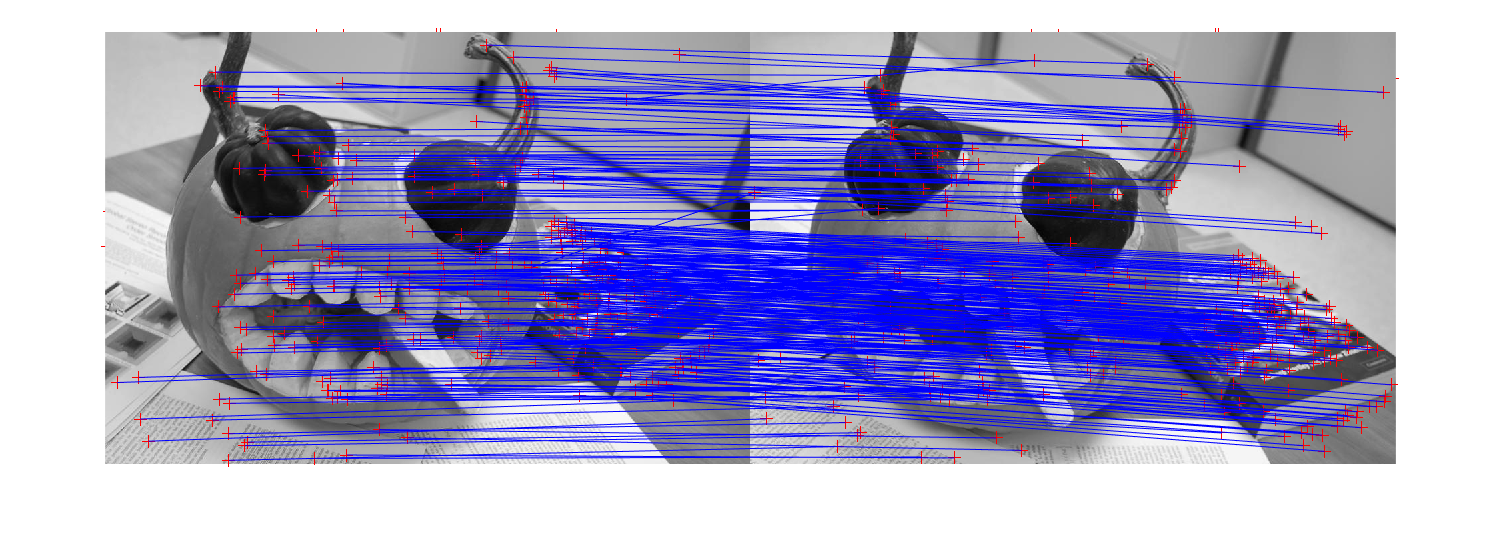
\includegraphics[width=1\linewidth, trim = {3cm 1cm 3cm 1cm}, clip]{C:/Users/Anton/Desktop/ETH_books/CV/CV-Lab-Model-Fitting/CV-Lab-Model-Fitting/src/epipolar_geometry/res/z-5-10000}
			\caption{Adaptive RANSAC, 5 threshold, 472 iterations.}
		\end{minipage}
	\end{center}
\end{figure}
\begin{figure}[h!]
	\begin{center}
		\begin{minipage}[h]{0.9\linewidth}
			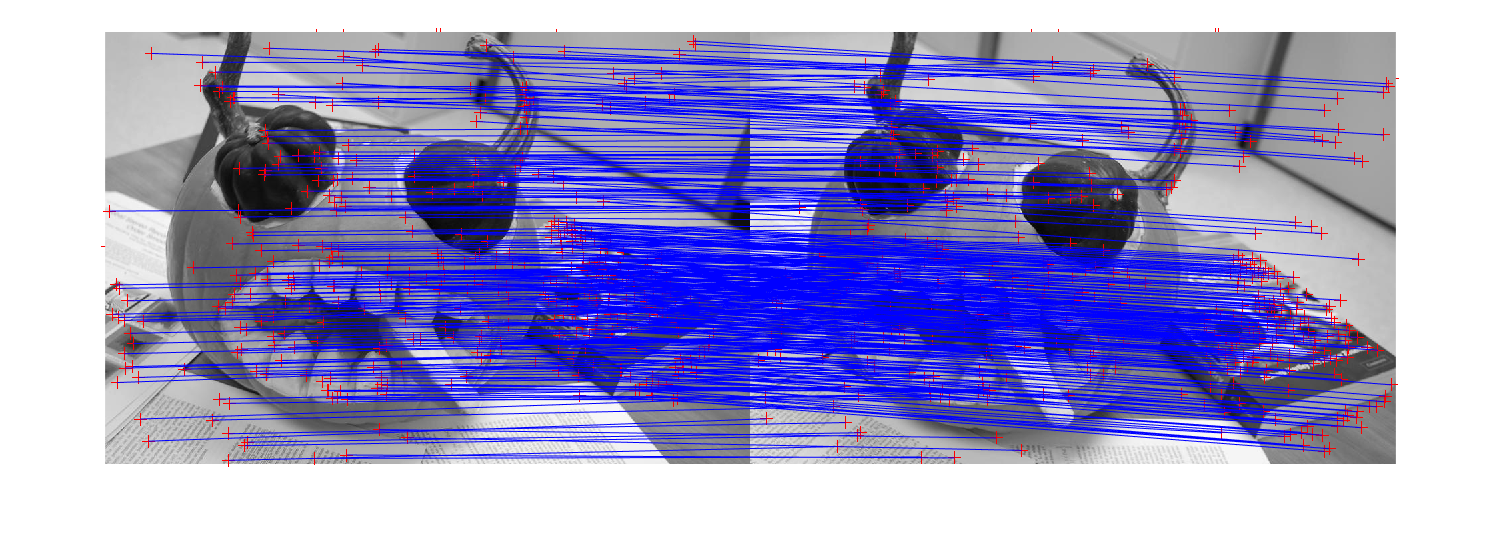
\includegraphics[width=1\linewidth, trim = {3cm 1cm 3cm 1cm}, clip]{C:/Users/Anton/Desktop/ETH_books/CV/CV-Lab-Model-Fitting/CV-Lab-Model-Fitting/src/epipolar_geometry/res/z-20-10000}
			\caption{Adaptive RANSAC, 20 threshold, 77 iterations.}
		\end{minipage}
	\end{center}
\end{figure}
\begin{figure}[h!]
	\begin{center}
		\begin{minipage}[h]{0.9\linewidth}
			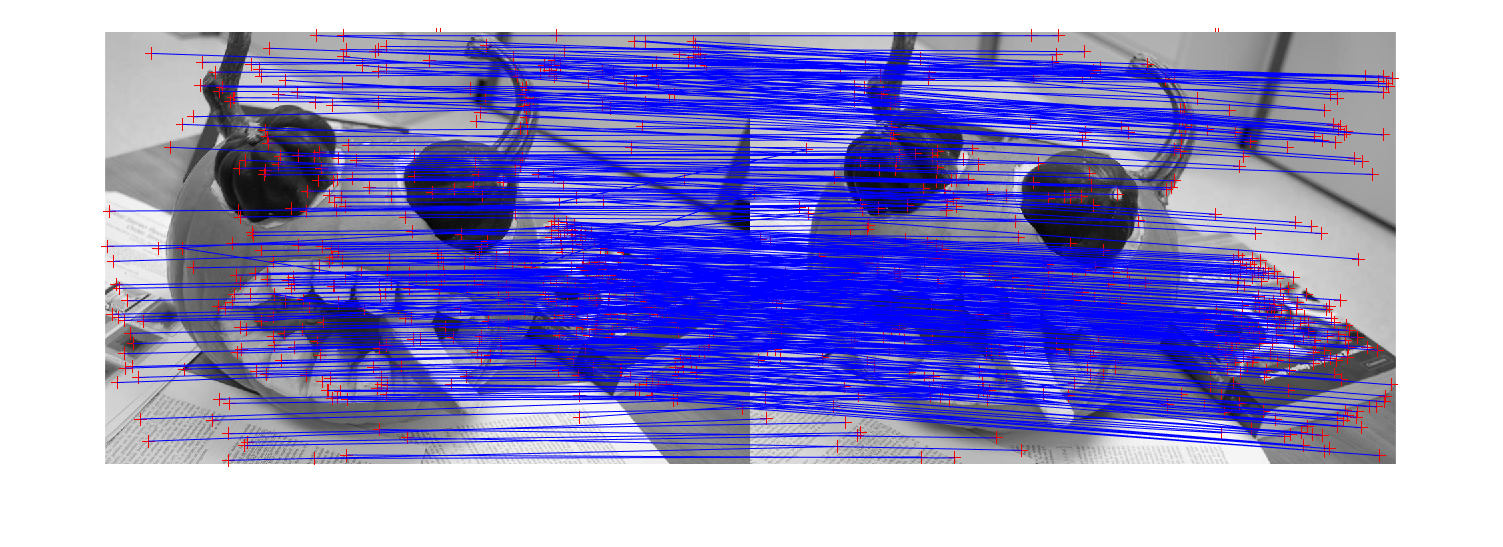
\includegraphics[width=1\linewidth, trim = {3cm 1cm 3cm 1cm}, clip]{C:/Users/Anton/Desktop/ETH_books/CV/CV-Lab-Model-Fitting/CV-Lab-Model-Fitting/src/epipolar_geometry/res/z-100-10000}
			\caption{Adaptive RANSAC, 100 threshold, 18 iterations.}
		\end{minipage}
	\end{center}
\end{figure}

\begin{figure}[h!]
	\begin{center}
		\begin{minipage}[h]{0.9\linewidth}
			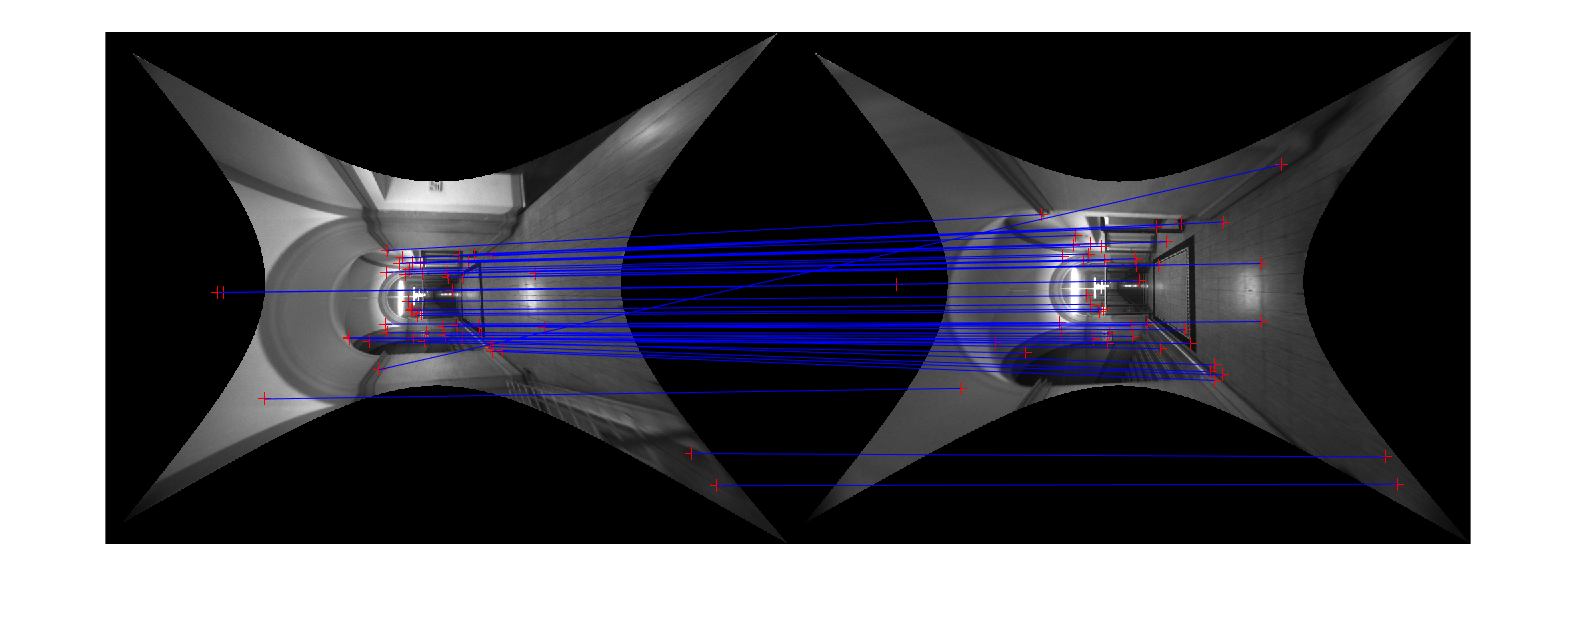
\includegraphics[width=1\linewidth, trim = {3cm 1cm 3cm 1cm}, clip]{C:/Users/Anton/Desktop/ETH_books/CV/CV-Lab-Model-Fitting/CV-Lab-Model-Fitting/src/epipolar_geometry/res/x-20-1000}
			\caption{RANSAC, 20 threshold, 1000 iterations.}
		\end{minipage}
	\end{center}
\end{figure}
\begin{figure}[h!]
	\begin{center}
		\begin{minipage}[h]{0.9\linewidth}
			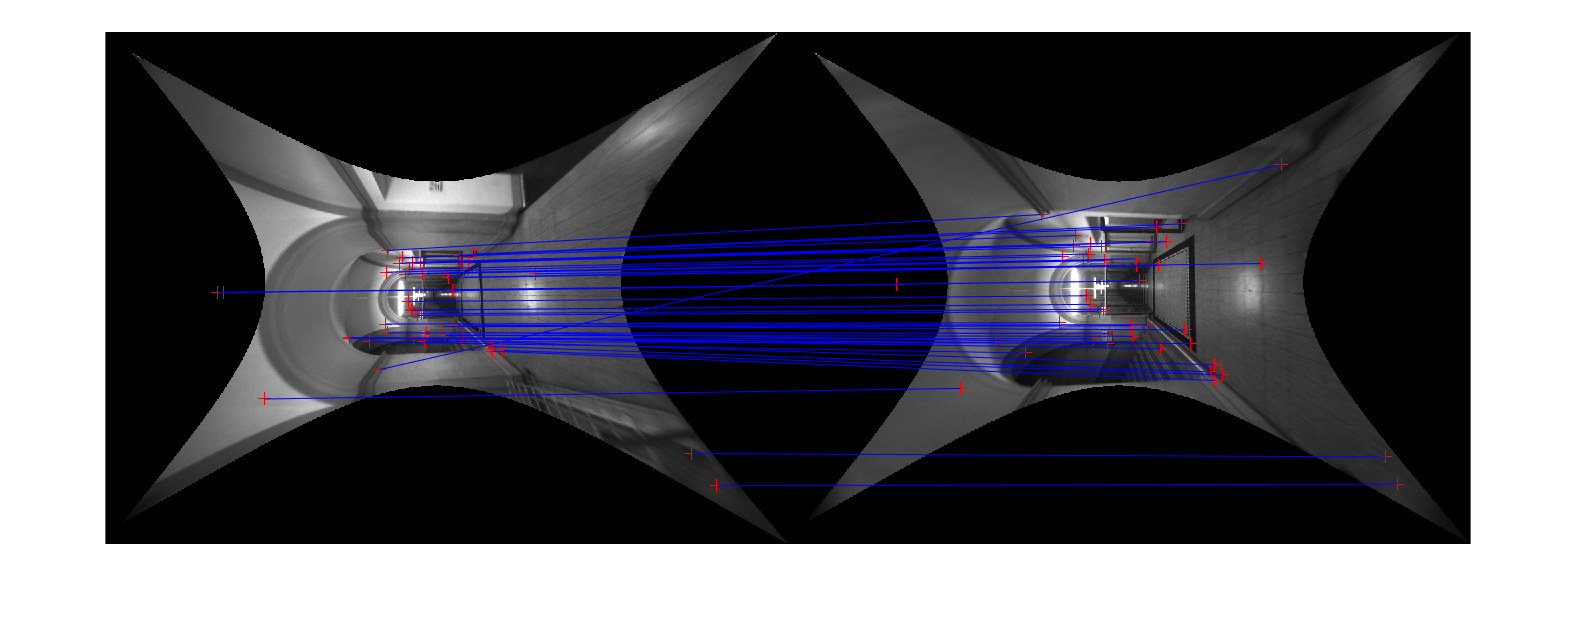
\includegraphics[width=1\linewidth, trim = {3cm 1cm 3cm 1cm}, clip]{C:/Users/Anton/Desktop/ETH_books/CV/CV-Lab-Model-Fitting/CV-Lab-Model-Fitting/src/epipolar_geometry/res/x-20-10000}
			\caption{Adaptive RANSAC, 20 threshold, 695 iterations.}
		\end{minipage}
	\end{center}
\end{figure}
\begin{figure}[h!]
	\begin{center}
		\begin{minipage}[h]{0.9\linewidth}
			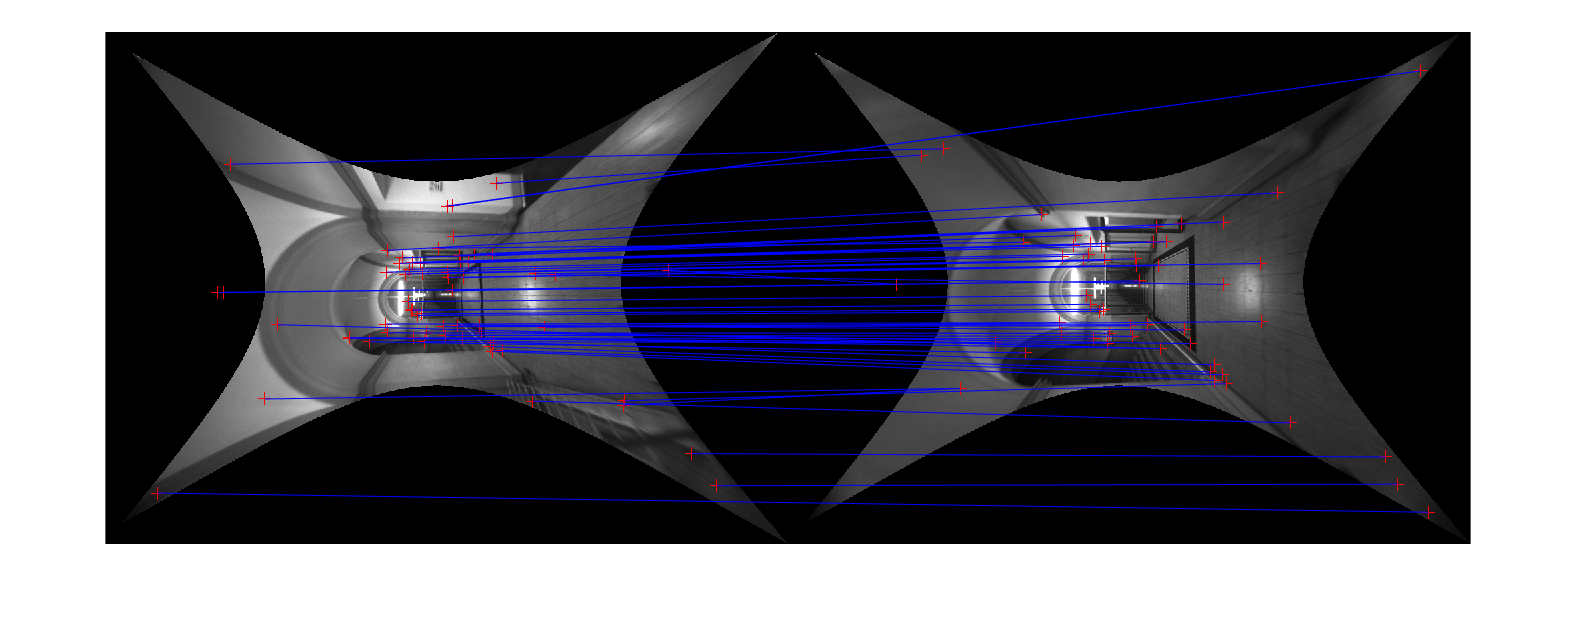
\includegraphics[width=1\linewidth, trim = {3cm 1cm 3cm 1cm}, clip]{C:/Users/Anton/Desktop/ETH_books/CV/CV-Lab-Model-Fitting/CV-Lab-Model-Fitting/src/epipolar_geometry/res/x-100-1000}
			\caption{RANSAC, 100 threshold, 1000 iterations.}
		\end{minipage}
	\end{center}
\end{figure}
\begin{figure}[h!]
	\begin{center}
		\begin{minipage}[h]{0.9\linewidth}
			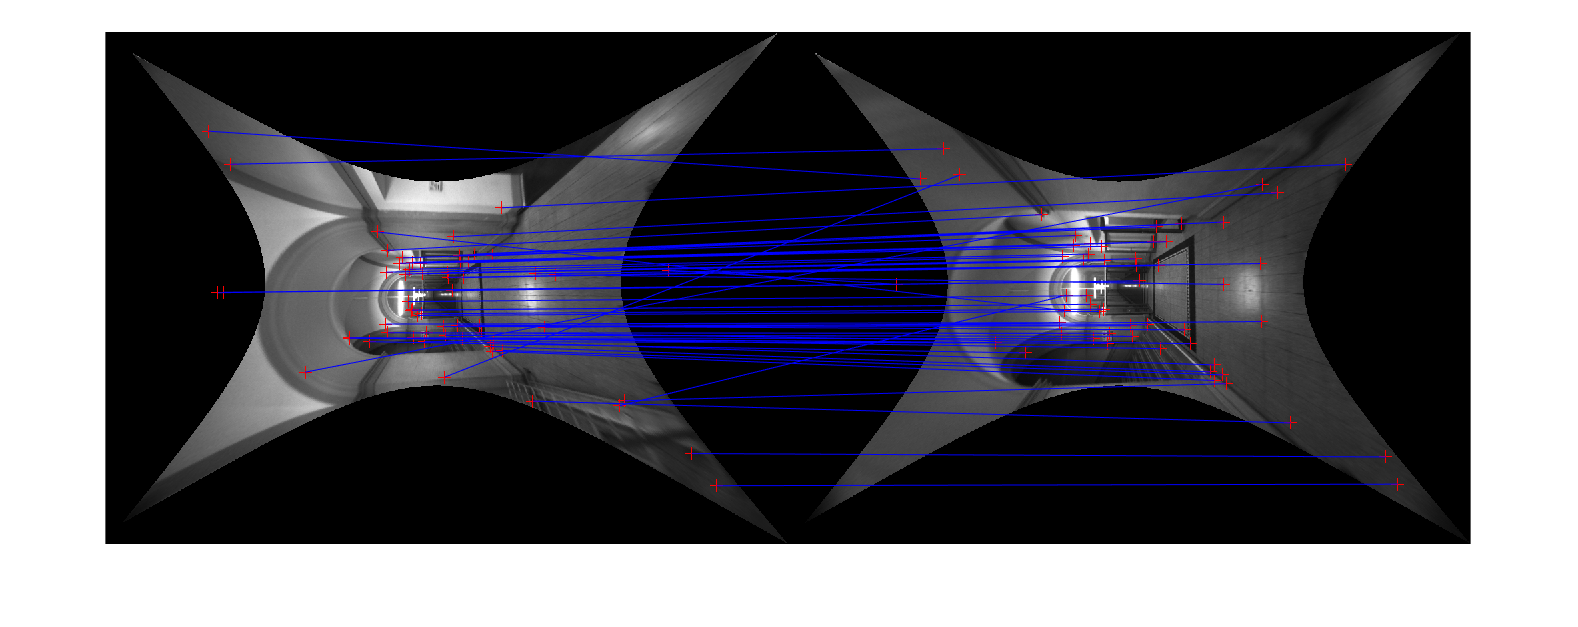
\includegraphics[width=1\linewidth, trim = {3cm 1cm 3cm 1cm}, clip]{C:/Users/Anton/Desktop/ETH_books/CV/CV-Lab-Model-Fitting/CV-Lab-Model-Fitting/src/epipolar_geometry/res/x-100-10000}
			\caption{Adaptive RANSAC, 100 threshold, 137 iterations. Amount and quality (though bad here, too big threshold) of inliers is the same as was with non-adaptive algorithm, but less iterations, that is beneficial}
		\end{minipage}
	\end{center}
\end{figure}

\begin{center}
	\textbf{Conclusion}
\end{center}
\begin{enumerate}
	\item Amount and quality of inliers are the same as was with non-adaptive algorithm, but less iterations, that is computationally beneficial.
	
	\item  At not more or less <<translational>> images adaptive RANSAC helps more in terms of number of iterations, because in these images present more true correspondent patches and greater number of inliers reduces number of iterations to reasonable amount. In example <<rect>> till threshold 100 there are still 1000 iterations, so adaptive algorithm doesn't change anything.
	
	\item Also, in corridor scene error it is more possible when points are on the different <<poles>> in relation to the epipole (but near the epipolar line), what induces scene-specific errors. 
\end{enumerate}





\end{document}